% =========================================================
% CHAPTER 5 - RESULTS
% =========================================================

\chapter{Results and Discussion}
\label{chap:experimental_results}

This chapter presents and discusses the results obtained from the experimental configurations described in Chapter~\ref{chap:experimental_methodology}. The analysis follows the evaluation framework established in Section~\ref{sec:statistical_analysis}, distinguishing between the primary confirmatory analysis and the secondary descriptive outcomes. The complete numerical results from all the 27 experimental configurations are provided in Appendix~\ref{app:experimental_results}

\section{Balance Verification}
\label{sec:balance_verification}

Firstly, after generating the balanced training subsets, a brief verification was carried out to confirm that the balancing procedure lead to the intended redistribution of samples. This verification was conducted for every experimental configuration.

For each balanced subset, the achieved counts in severe hypoglycemia, hypoglycemia, normoglycemia, hyperglycemia, and severe hyperglycemia were compared with the theoretical target counts calculated by the balancing module. The same verification was performed for all 27 combinations of dataset, balancing method, and target distribution. The achieved counts matched the calculated targets "exactly". The only minor differences arose when proportional targets had to be converted into integer sample counts -- the remaining samples caused by rounding were assigned to the normoglycemic range so that the final combined size remained correct. The complete logs where all the configurations targets appear can be found in Appendix~\ref{app:experimental_results}.

Once the correctness of the range-level counts had been confirmed, the resulting target-value distributions were inspected graphically.

\begin{quote}
\small
\textit{\textbf{Note.} The REPLACE-BG dataset is used in this section as a representative example, since the corresponding distributions for the other datasets were also examined and confirmed to show analogous behaviour. The complete set of figures is provided in Appendix~\ref{app:experimental_results}. For each target configuration, the distributions obtained through random resampling, SMOTER, and SMOGN are presented together. This allows the effect of the balancing level to be distinguished from that of the sampling method. Although the three methods were configured to reach the same range-level counts, they differ in how samples are distributed within each glycemic range.}
\end{quote}


\begin{figure}[htbp]
    \centering

    \begin{subfigure}{0.9\textwidth}
        \centering
        
\includegraphics[width=\textwidth]{images/balanced_distribution/REPLACE-BG_random_normalized.png}
    \end{subfigure}

    \vspace{0.5cm}

    \begin{subfigure}{0.9\textwidth}
        \centering
        
\includegraphics[width=\textwidth]{images/balanced_distribution/REPLACE-BG_smoter_normalized.png}
    \end{subfigure}

    \vspace{0.5cm}

    \begin{subfigure}{0.9\textwidth}
        \centering
        
\includegraphics[width=\textwidth]{images/balanced_distribution/REPLACE-BG_smogn_normalized.png}
    \end{subfigure}

    \caption{Balanced distribution on normalized target, methods comparison.}
    \label{fig:balanced_normalized_methods_comparison}
\end{figure}

Figure~\ref{fig:balanced_normalized_methods_comparison} presents the normalized configuration. This configuration introduces the smallest change, and the resulting distributions remain relatively close to the original glucose distribution, indicating that only limited oversampling or undersampling was required under this configuration. The three balancing methods produce very similar overall shapes, indicating that none of them introduces a systematic concentration of samples within particular regions of the glucose range.

\begin{figure}[htbp]
    \centering

    \begin{subfigure}{0.9\textwidth}
        \centering
        
\includegraphics[width=\textwidth]{images/balanced_distribution/REPLACE-BG_random_semi.png}
    \end{subfigure}

    \vspace{0.5cm}

    \begin{subfigure}{0.9\textwidth}
        \centering
        
\includegraphics[width=\textwidth]{images/balanced_distribution/REPLACE-BG_smoter_semi.png}
    \end{subfigure}

    \vspace{0.5cm}

    \begin{subfigure}{0.9\textwidth}
        \centering
        
\includegraphics[width=\textwidth]{images/balanced_distribution/REPLACE-BG_smogn_semi.png}
    \end{subfigure}

    \caption{Balanced distribution on normalized target, methods comparison.}
    \label{fig:balanced_semi_methods_comparison}
\end{figure}

Figure~\ref{fig:balanced_semi_methods_comparison} presents the semi-balanced configuration. In this case, the redistribution is more noticeable: the minority ranges gain representation and the predominance of normoglycemia is reduced, while the overall distribution remains intentionally unequal. The configuration therefore represents an intermediate condition between the normalized and fully balanced distributions. The three methods also maintain comparable range-level shapes

\begin{figure}[htbp]
    \centering

    \begin{subfigure}{0.9\textwidth}
        \centering
        
\includegraphics[width=\textwidth]{images/balanced_distribution/REPLACE-BG_random_full.png}
    \end{subfigure}

    \vspace{0.5cm}

    \begin{subfigure}{0.9\textwidth}
        \centering
        
\includegraphics[width=\textwidth]{images/balanced_distribution/REPLACE-BG_smoter_full.png}
    \end{subfigure}

    \vspace{0.5cm}

    \begin{subfigure}{0.9\textwidth}
        \centering
        
\includegraphics[width=\textwidth]{images/balanced_distribution/REPLACE-BG_smogn_full.png}
    \end{subfigure}

    \caption{Balanced distribution on normalized target, methods comparison.}
    \label{fig:balanced_full_methods_comparison}
\end{figure}

Figure~\ref{fig:balanced_full_methods_comparison} presents the fully balanced configuration, which produces the strongest modification. The three methods also maintain comparable range-level shapes. Although each glycemic range contains the same total number of training windows, the five ranges have substantially different widths. Consequently, concentrating the same number of samples within a narrower interval produces much higher frequencies per glucose value, explaining the pronounced peaks in TBR.

Abrupt changes can also be observed at ranges limits: 54, 70, 181, and 251 mg/dL. These discontinuities are expected because each glycemic range is processed independently and receives a different sampling factor.

Overall, the verification confirmed that all balanced subsets matched their intended target counts. Also, it showed that the overall redistribution across the five glycemic ranges remains consistent, confirming that the balancing level determines the quantity of samples assigned to each range, while suggesting that the chosen balancing method hardly -- does not almost -- affects their internal distribution.

% ============================================================
% DIATREND
% ============================================================

\section{DiaTrend Results}
\label{sec:diatrend_results}

\subsection{Primary Statistical Test}
\label{subsec:diatrend_primary_analysis}

As defined in Section~\ref{sec:statistical_analysis}, the statistical analysis evaluates whether full balancing improves the proportion of clinically acceptable predictions in severe hypoglycemia, \(AB_{\mathrm{TBR_2}}\), relative to the corresponding \texttt{NORMALIZED\_BASELINE} configuration.

First, the difference between the fully balanced and normalized configurations was first calculated independently for each of the methods and cross-validation folds. Then, the three method-specific differences were averaged within each fold according to Equation~\ref{eq:fold_mean_delta_ab_tbr2}. The resulting values, presented in Table~\ref{tab:diatrend_fold_primary_effect} in percentage points, constitue the five fold-level observations used in the Student's \(t\)-test.

\begin{table}[htbp]
    \centering
    \caption{DiaTrend fold-level prediction performance for the primary clinical outcome.}
    \label{tab:diatrend_fold_primary_effect}
    \begin{tabular}{cccc}
        \toprule
        \textbf{Fold}
        & \textbf{Normalized A+B}
        & \textbf{Full A+B}
        & \(\boldsymbol{\Delta}\) \textbf{A+B} \\
        \midrule
        1 & 0.36\% & 47.90\% & +47.54 pp \\
        2 & 1.17\% & 59.42\% & +58.25 pp \\
        3 & 6.71\% & 68.59\% & +61.89 pp \\
        4 & 0.02\% & 79.65\% & +79.62 pp \\
        5 & 7.55\% & 79.01\% & +71.46 pp \\
        \midrule
        \textbf{Mean}
        & \textbf{3.16\%}
        & \textbf{66.91\%}
        & \textbf{+63.75 pp} \\
        \bottomrule
    \end{tabular}
\end{table}

Full balancing produced a positive improvement in every cross-validation fold, with values that range from \(47.54\) to \(79.62\) percentage points. Moreover, all 15 individual method--fold comparisons ~\ref{app:experimental_results} were positive, which suggests that this effect is also consistent across balancing methods. The five observations used in the statistical test are therefore:

\begin{equation}
d_f
\in
\{
47.54,\,
58.25,\,
61.89,\,
79.62,\,
71.46
\}
\text{ pp}.
\end{equation}

Their mean and standard deviation were:

\begin{equation}
\overline{d}
=
63.75
\text{ pp},
\end{equation}

\begin{equation}
s_d
=
12.33
\text{ pp}.
\end{equation}

Applying the one-sided paired Student's \(t\)-test defined in Section~\ref{subsec:statistical_hypotheses} produced the following statistic:

\begin{equation}
t
=
\frac{63.75}{12.33/\sqrt{5}}
=
11.57.
\end{equation}

With \(n-1=4\) degrees of freedom, the corresponding one-sided \(p\)-value was:

\begin{equation}
p
=
0.00016.
\end{equation}

Since:

\begin{equation}
p < \alpha
\qquad
(0.00016 < 0.01),
\end{equation}

the null hypothesis defined in Equation~\ref{eq:null_hypothesis_tbr2} can be be rejected for DiaTrend with a considerable degree of confidence.

Additionally, this statistical significance is accompanied by a substantial effect magnitude. Across the five folds, full balancing increased \(AB_{\mathrm{TBR_2}}\) by an average of \(63.75\) percentage points: the mean value increased from \(3.16\%\) under the normalized baseline to \(66.91\%\) under full balancing.

The improvement was also consistent across the complete experimental configuration. Every fold showed a positive mean difference, and every individual comparison involving random resampling, SMOTER, or SMOGN favoured full balancing. Consequently, the result does not appear to depend on a particular balancing method or cross-validation partition.

Therefore, the primary statistical result supports the study hypothesis for DiaTrend: \textbf{increasing the representation of rare glycemic ranges through full balancing produces a statistically significant and clinically substantial improvement in the proportion of acceptable predictions in severe hypoglycemia}. The remaining secondary outcomes must subsequently determine whether this benefit is accompanied by acceptable changes in the other glycemic ranges.

\subsection{Secondary Outcomes}
\label{subsec:diatrend_secondary_outcomes}

Together with the primary statistical analysis, a secondary analyses was performed to study the impact of balancing in the rest of regression and clinical metrics. A single statistical test, narrowed to a very particular although critical metric, should not be considered enough to determine the full effect.

\begin{quote}
\small
\textit{\textbf{Note.} The secondary analysis uses the aggregate results obtained after combining the predictions from all folds for each experimental configuration. Consequently, the aggregate percentages reported in this subsection do not necessarily coincide exactly with the unweighted mean of the five fold-level percentages used in the previous statistical test. In any case, full results can be checked in Appendix~\ref{app:experimental_results}. Considering the large number of experiments and the corresponding performance metrics, for the scope if this secondary analysis, results are presented mostly summarized through their mean and descriptive standard deviation. Also, the normalized configuration remains the reference for interpreting the changes introduced by semi and full-balancing.}
\end{quote}

\subsubsection{Influence of the Balancing Method}
\label{subsubsec:diatrend_method_influence}

Table~\ref{tab:diatrend_method_influence} presents a condensed comparison between target distributions of some of the main global metrics. Each value represents the mean and standard deviation computed across the three method-specific aggregate results.

\begin{table}[htbp]
    \centering
    \caption{Main DiaTrend results.}
    \label{tab:diatrend_method_influence}
    \resizebox{\textwidth}{!}{
    \begin{tabular}{lcccccc}
        \toprule
        \textbf{Target}
        & \textbf{Entire RMSE}
        & \textbf{Entire A+B}
        & \textbf{TBR$_2$ RMSE}
        & \textbf{TBR$_2$ A+B}
        & \textbf{TBR$_1$ RMSE}
        & \textbf{TBR$_1$ A+B} \\
        \midrule
        Normalized
        & \(46.69 \pm 0.10\)
        & \(95.23 \pm 0.01\)
        & \(64.46 \pm 0.97\)
        & \(3.74 \pm 1.81\)
        & \(52.20 \pm 0.41\)
        & \(1.60 \pm 0.49\) \\

        Semi-balanced
        & \(46.41 \pm 0.14\)
        & \(96.02 \pm 0.02\)
        & \(51.33 \pm 0.58\)
        & \(35.73 \pm 1.56\)
        & \(42.79 \pm 0.33\)
        & \(28.99 \pm 1.34\) \\

        Fully balanced
        & \(49.92 \pm 0.17\)
        & \(96.09 \pm 0.03\)
        & \(41.07 \pm 0.85\)
        & \(72.68 \pm 0.35\)
        & \(35.14 \pm 0.56\)
        & \(70.35 \pm 0.25\) \\
        \bottomrule
    \end{tabular}
    }
\end{table}

Compared with the differences between target distributions, the variability across methods was consistently insignificant. For example, when analyzing global performance, the standard deviation across methods remained below \(0.18\) mg/dL for RMSE and below \(0.03\) percentage points for A+B. Under full balancing, TBR$_2$ A+B ranged only from \(72.27\%\) to \(73.13\%\), and TBR$_1$ A+B ranged from \(70.03\%\) to \(70.65\%\).

The only considerable "method-related" variability was found in the normalized hypoglycemic results, where the model is actually known to perform poorly. But even in this case, the difference between methods remained considerably smaller than the improvements obtained by changing the balancing intensity.

These results do not necessarily prove that the three methods are equivalent, since no formal statistically test was performed. However, they clearly show that the selected target distribution -- or balancing intensity -- has a much higher influence in the predictive performance than the particular oversampling method.

\subsubsection{Effect of Balancing Intensity in Hypoglycemia}
\label{subsubsec:diatrend_hypoglycemia}

The hypoglycemic results -- which proved to have the most substantial improvements -- are also analyzed across the normalized, \textbf{semi-balanced}, and fully balanced configurations in order to determine how the predictive performance changes as the degree of balancing increases.

\begin{table}[htbp]
    \centering
    \caption{DiaTrend performance in the hypoglycemic ranges,
    averaged across balancing methods.}
    \label{tab:diatrend_hypoglycemia}
    \resizebox{\textwidth}{!}{
    \begin{tabular}{llccccc}
        \toprule
        \textbf{Target}
        & \textbf{Range}
        & \textbf{RMSE}
        & \textbf{MAE}
        & \textbf{A+B}
        & \textbf{Zone D}
        & \textbf{Zone E} \\
        \midrule
        Normalized & TBR$_2$
        & 64.46 & 59.07 & 3.74\% & 94.20\% & 2.05\% \\
        Semi-balanced & TBR$_2$
        & 51.33 & 39.29 & \textbf{35.73\%} & 61.98\% & 2.28\% \\
        Fully balanced & TBR$_2$
        & \textbf{41.07} & 24.66 & \textbf{72.68\%} & 25.16\% & 2.16\% \\
        \midrule
        Normalized & TBR$_1$
        & 52.20 & 46.48 & 1.60\% & 96.33\% & 2.06\% \\
        Semi-balanced & TBR$_1$
        & 42.79 & 30.94 & \textbf{28.99\%} & 68.71\% & 2.29\% \\
        Fully balanced & TBR$_1$
        & \textbf{35.14} & 19.07 & \textbf{70.35\%} & 27.39\% & 2.25\% \\
        \bottomrule
    \end{tabular}
    }
\end{table}

Table~\ref{tab:diatrend_hypoglycemia} summarizes some critical metrics for TBR for each of the balancing targets. Normalized target is presented as a reference. Zones B and C contained no predictions in these ranges, so A+B is equivalent to Zone A.

Semi-balancing resulted in a substantial intermediate improvement, relative to the normalized baseline: TBR$_2$ RMSE decreased by \(13.13\) mg/dL and A+B increased by \(31.99\%\); In TBR$_1$, RMSE decreased by \(9.41\) mg/dL and and A+B increased by \(27.39\%\). These clinical gains were mainly produced by a redistribution from Zone D into Zone A.

Full balancing intensified this effect: TBR$_2$ RMSE decreased by \(23.40\) mg/dL and A+B increased by \(68.93\%\); In TBR$_1$, RMSE decreased by \(17.07\) mg/dL and and A+B increased by \(68.75\%\). The redistribution from Zone D into Zone A was also similarly pronounced.

Semi-balancing therefore provided a valid intermediate response, and full balancing produced a substantially larger improvement in both numerical accuracy and clinical acceptability. While not formally proven with the corresponding statistical test, these results suggest that the predictive performance improves progressively as the degree of balancing increases -- at least up to a fully symmetrical distribution.

\begin{equation}
\label{eq:ordered_hypothesis_conjecture}
AB_{\mathrm{TBR}}^{(\mathrm{normalized})}
<
AB_{\mathrm{TBR}}^{(\mathrm{semi})}
<
AB_{\mathrm{TBR}}^{(\mathrm{full})}.
\end{equation}


\subsubsection{Global and Time-in-Range Trade-Off}
\label{subsubsec:diatrend_global_tir}

The improvement in hypoglycemia must also be interpreted together with its effect on global performance and TIR, which actually represents the most frequently observed glycemic range. Table~\ref{tab:diatrend_global_tir} summarizes these results.

\begin{table}[htbp]
    \centering
    \caption{Aggregate global and TIR performance in DiaTrend, averaged
    across balancing methods.}
    \label{tab:diatrend_global_tir}
    \resizebox{\textwidth}{!}{
    \begin{tabular}{llcccccc}
        \toprule
        \textbf{Target}
        & \textbf{Range}
        & \textbf{RMSE}
        & \textbf{MAE}
        & \textbf{A+B}
        & \textbf{Zone D}
        & \textbf{Zone E} \\
        \midrule
        Normalized & Entire
        & 46.69 & 34.26 & 95.23\% & 4.45\% & 0.04\% \\
        Semi-balanced & Entire
        & 46.41 & 33.55 & 96.02\% & 3.48\% & 0.13\% \\
        Fully balanced & Entire
        & \textbf{49.92} & 36.23 & 96.09\% & 2.67\% & 0.69\% \\
        \midrule
        Normalized & TIR
        & 29.13 & 21.36 & 99.50\% & \textbf{0.00\%} & \textbf{0.00\%} \\
        Semi-balanced & TIR
        & 32.43 & 23.27 & 99.33\% & \textbf{0.00\%} & \textbf{0.00\%} \\
        Fully balanced & TIR
        & \textbf{38.23} & 28.21 & 99.01\% & \textbf{0.00\%} & \textbf{0.00\%} \\
        \bottomrule
    \end{tabular}
    }
\end{table}

Semi-balancing mostly preserved global numerical performance in comparison with the normalized baseline. Global RMSE decreased by \(0.28\) mg/dL and A+B increased by \(0.79\) percentage points. Therefore, its hypoglycemic improvements were not accompanied by a general deterioration in the aggregate metrics.

The main cost of semi-balancing appeared in TIR, where RMSE increased by \(3.30\) mg/dL. However, TIR A+B decreased by only \(0.17\) percentage points and still remained above \(99\%\).

Full balancing introduced a more pronounced numerical trade-off. Global RMSE increased by \(3.23\) mg/dL and MAE by \(1.97\) mg/dL, relative to the normalized baseline. Nevertheless, global A+B increased by \(0.86\) percentage points.

The largest numerical deterioration of full balancing appeared in TIR, where RMSE was increased by \(9.10\) mg/dL and MAE by \(6.85\) mg/dL. Nevertheless, IR A+B decreased by only \(0.49\) percentage points and remained at \(99.01\%\). Moreover, no TIR predictions entered Zones D or E.

The deterioration, both in TIR and globally, was therefore primarily numerical rather than
clinical: while predictions in this ranges became less precise, they remained almost entirely
within clinically acceptable regions.

\subsubsection{Hyperglycemic Ranges Performance}
\label{subsubsec:diatrend_hyperglycemia}

The effects in TAR were also studied and found to be positive, althoguh they slightly differ between moderate and severe hyperglycemia, as shown in Table~\ref{tab:diatrend_hyperglycemia}.

\begin{table}[htbp]
    \centering
    \caption{Aggregate DiaTrend performance in the hyperglycemic ranges,
    averaged across balancing methods.}
    \label{tab:diatrend_hyperglycemia}
    \resizebox{\textwidth}{!}{
    \begin{tabular}{llccccc}
        \toprule
        \textbf{Target}
        & \textbf{Range}
        & \textbf{RMSE}
        & \textbf{MAE}
        & \textbf{A+B}
        & \textbf{Zone D}
        & \textbf{Zone E} \\
        \midrule
        Normalized & TAR$_1$
        & 45.41 & 36.13 & 97.37\% & 2.54\% & 0.00\% \\
        Semi-balanced & TAR$_1$
        & 45.84 & 34.72 & 97.49\% & 2.13\% & 0.26\% \\
        Fully balanced & TAR$_1$
        & \textbf{50.64} & 36.82 & \textbf{95.84\%} & 2.02\% & \textbf{2.02\%} \\
        \midrule
        Normalized & TAR$_2$
        & 77.32 & 65.72 & 89.24\% & 10.76\% & 0.00\% \\
        Semi-balanced & TAR$_2$
        & 72.91 & 60.38 & 91.00\% & 8.96\% & 0.05\% \\
        Fully balanced & TAR$_2$
        & 73.21 & 59.22 & 90.89\% & 8.72\% & 0.39\% \\
        \bottomrule
    \end{tabular}
    }
\end{table}

Semi-balancing had only a limited impact on TAR$_1$: RMSE increased by \(0.43\) mg/dL, and A+B increased by \(0.11\) percentage points. TAR$_2$ improved more clearly: RMSE
decreased by \(4.41\) mg/dL, Zone D by \(1.80\) percentage points, and A+B increased by \(1.76\) percentage points.

Full balancing maintained most of the improvement in TAR$_2$. Relative to
the normalized baseline, RMSE decreased by \(4.11\) mg/dL, and Zone D by \(2.04\) percentage points. A+B increased by \(1.65\) percentage points. In contrast, TAR$_1$ presented a localized deterioration: RMSE increased by \(5.23\) mg/dL and A+B decreased by \(1.54\) percentage points. Although Zone A increased by \(2.05\) percentage points and Zone D decreased by \(0.52\) percentage points, Zone E increased from zero to \(2.02\%\). This adverse effect should therefore be considered in the overall interpretation of full balancing.

Overall, although some deterioration was introduced in TAR$_1$, it remained considerably smaller than the improvements achieved in TBR$_2$ and TBR$_1$. Moreover, severe hyperglycemia benefited from both semi-balancing and full balancing.

\subsubsection{Clarke Error Grid Interpretation}
\label{subsubsec:diatrend_clarke_interpretation}

Figures~\ref{fig:diatrend_clarke_semi} and \ref{fig:diatrend_clarke_full} present representative Clarke Error Grids for the semi-balanced and fully balanced resampling configurations, while Figure~\ref{fig:diatrend_clarke_normalized} is presented as the baseline for comparison, as described in Chapter~\ref{chap:experimental_methodology}. Having shown that the three balanding methods produce similar results, random resampling is the selected method for visualization because it represent the most simple approach.

\begin{figure}[htbp]
    \centering
    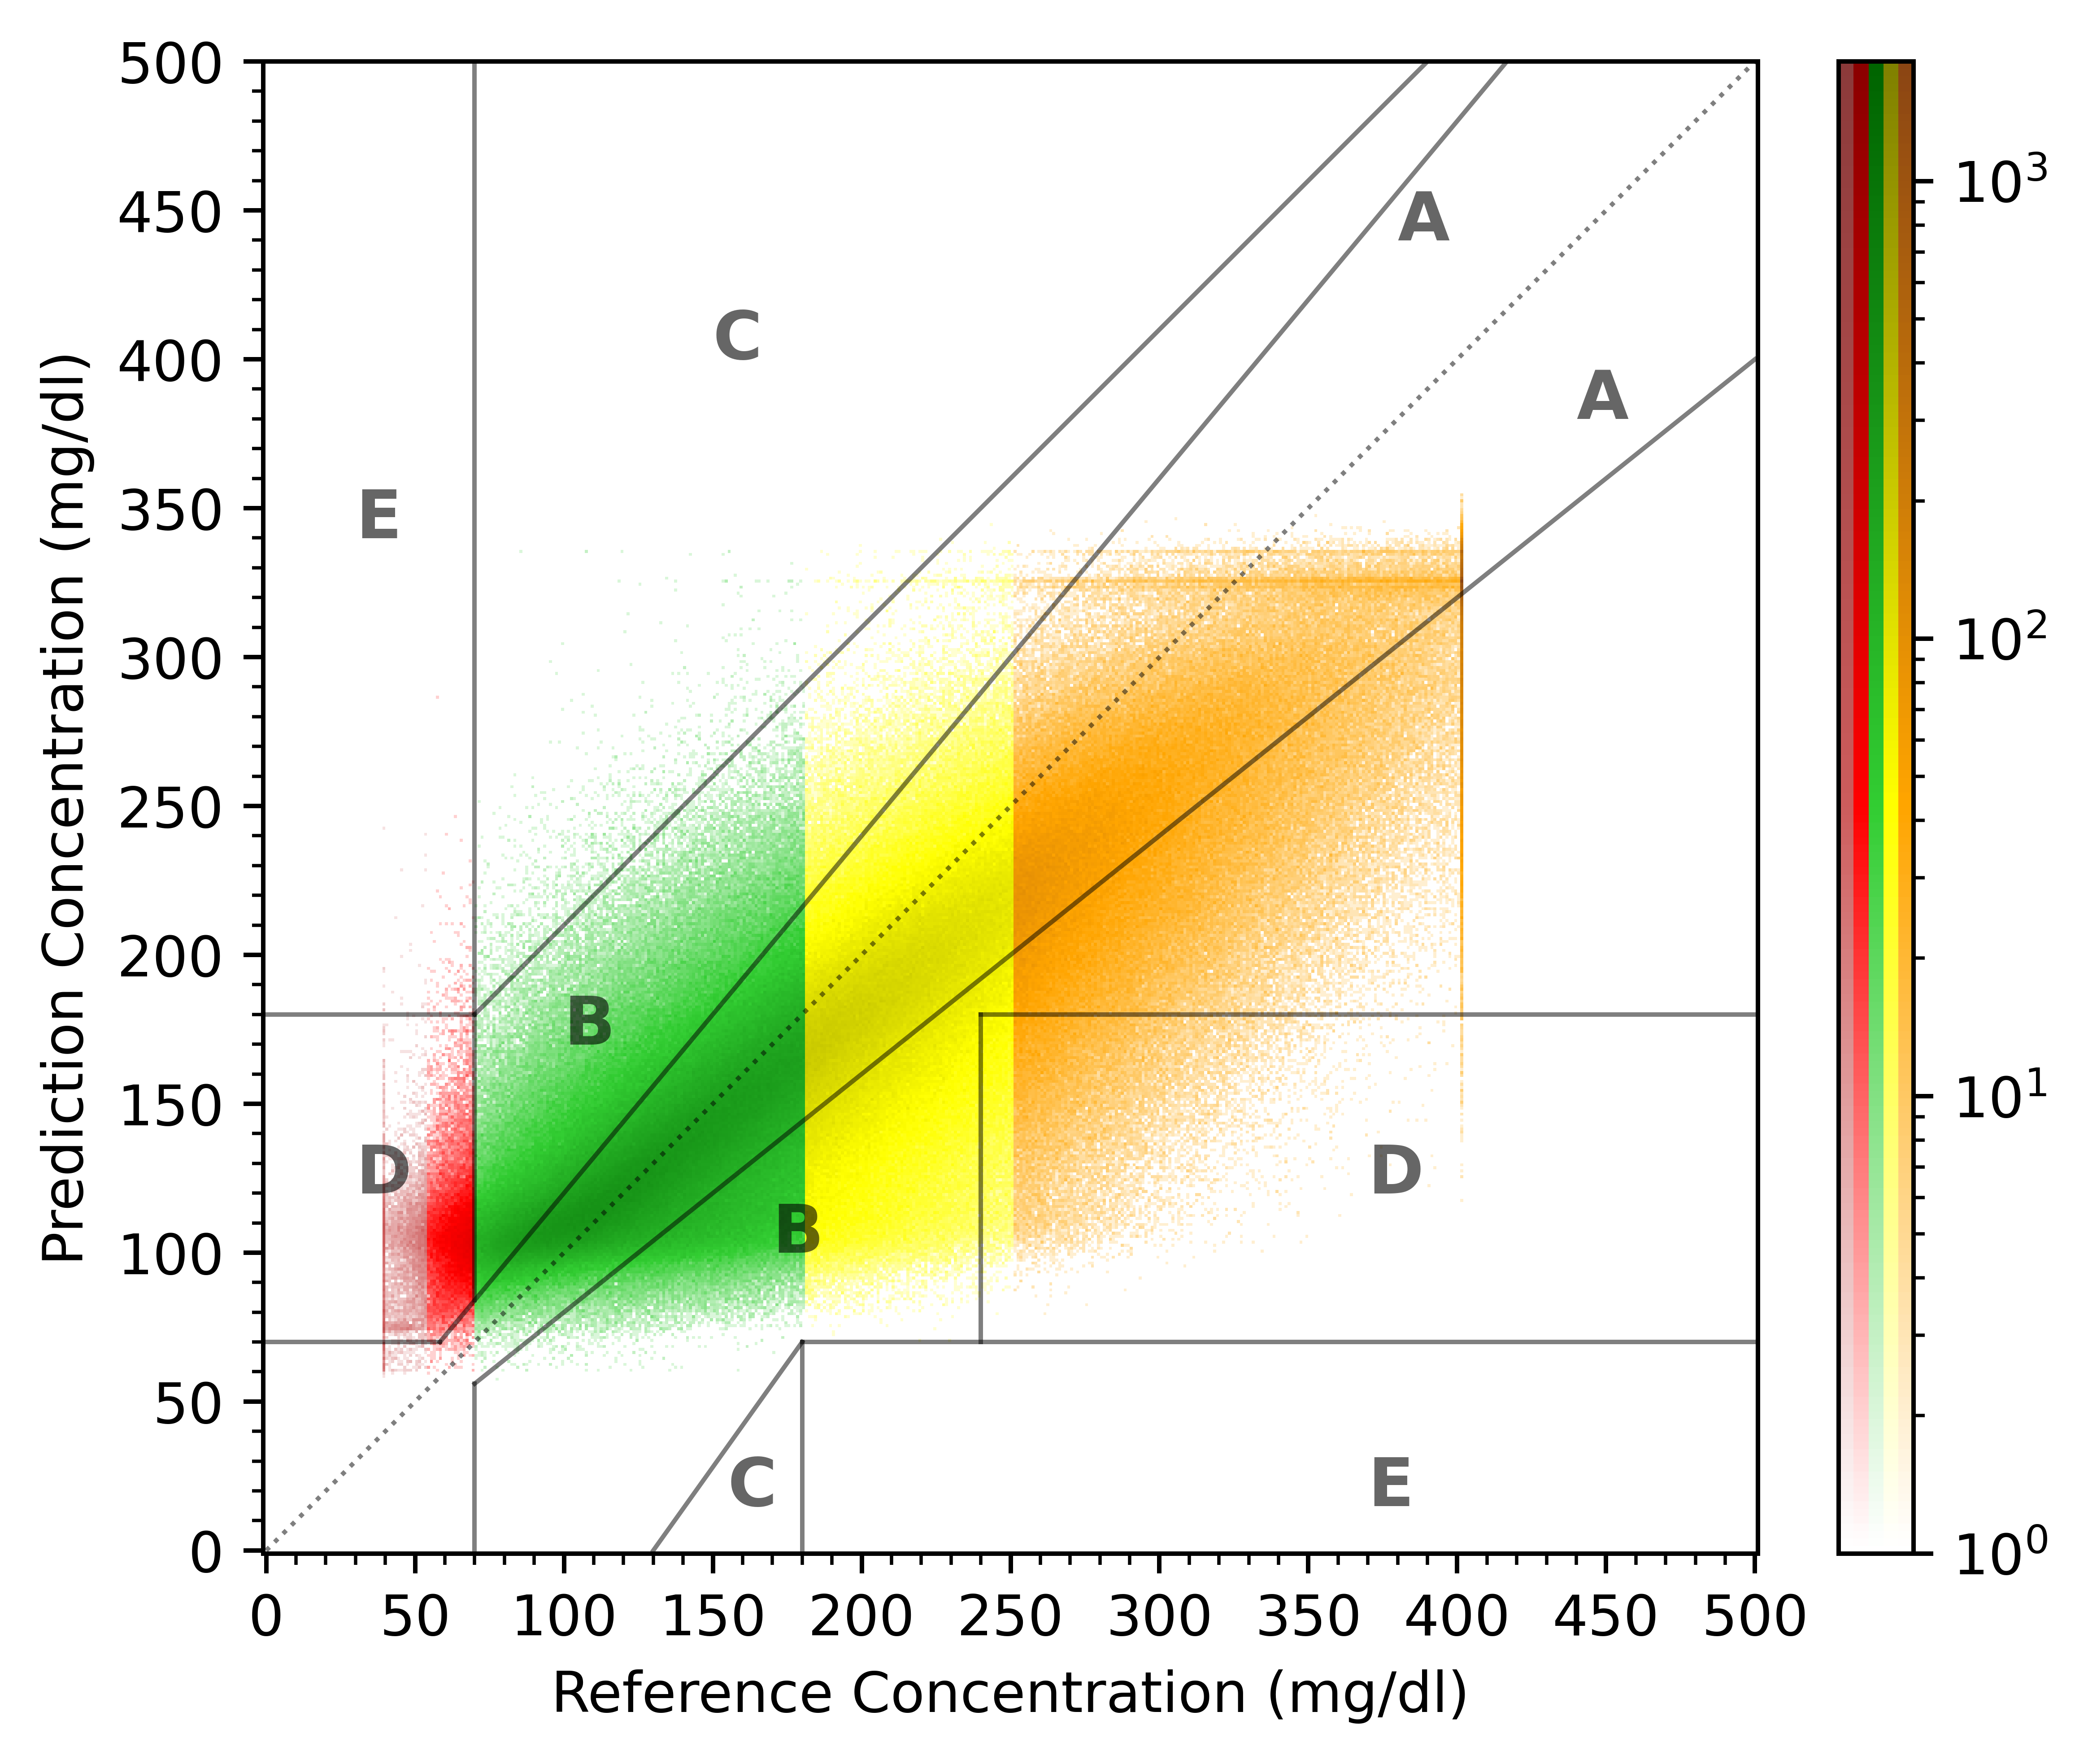
\includegraphics[width=0.82\textwidth]{images/CEGA_Diatrend/DiaTrend_random_normalized.png}
    \caption{Clarke Error Grid for DiaTrend using random resampling and
    the normalized baseline target distribution.}
    \label{fig:diatrend_clarke_normalized}
\end{figure}

\begin{figure}[htbp]
    \centering
    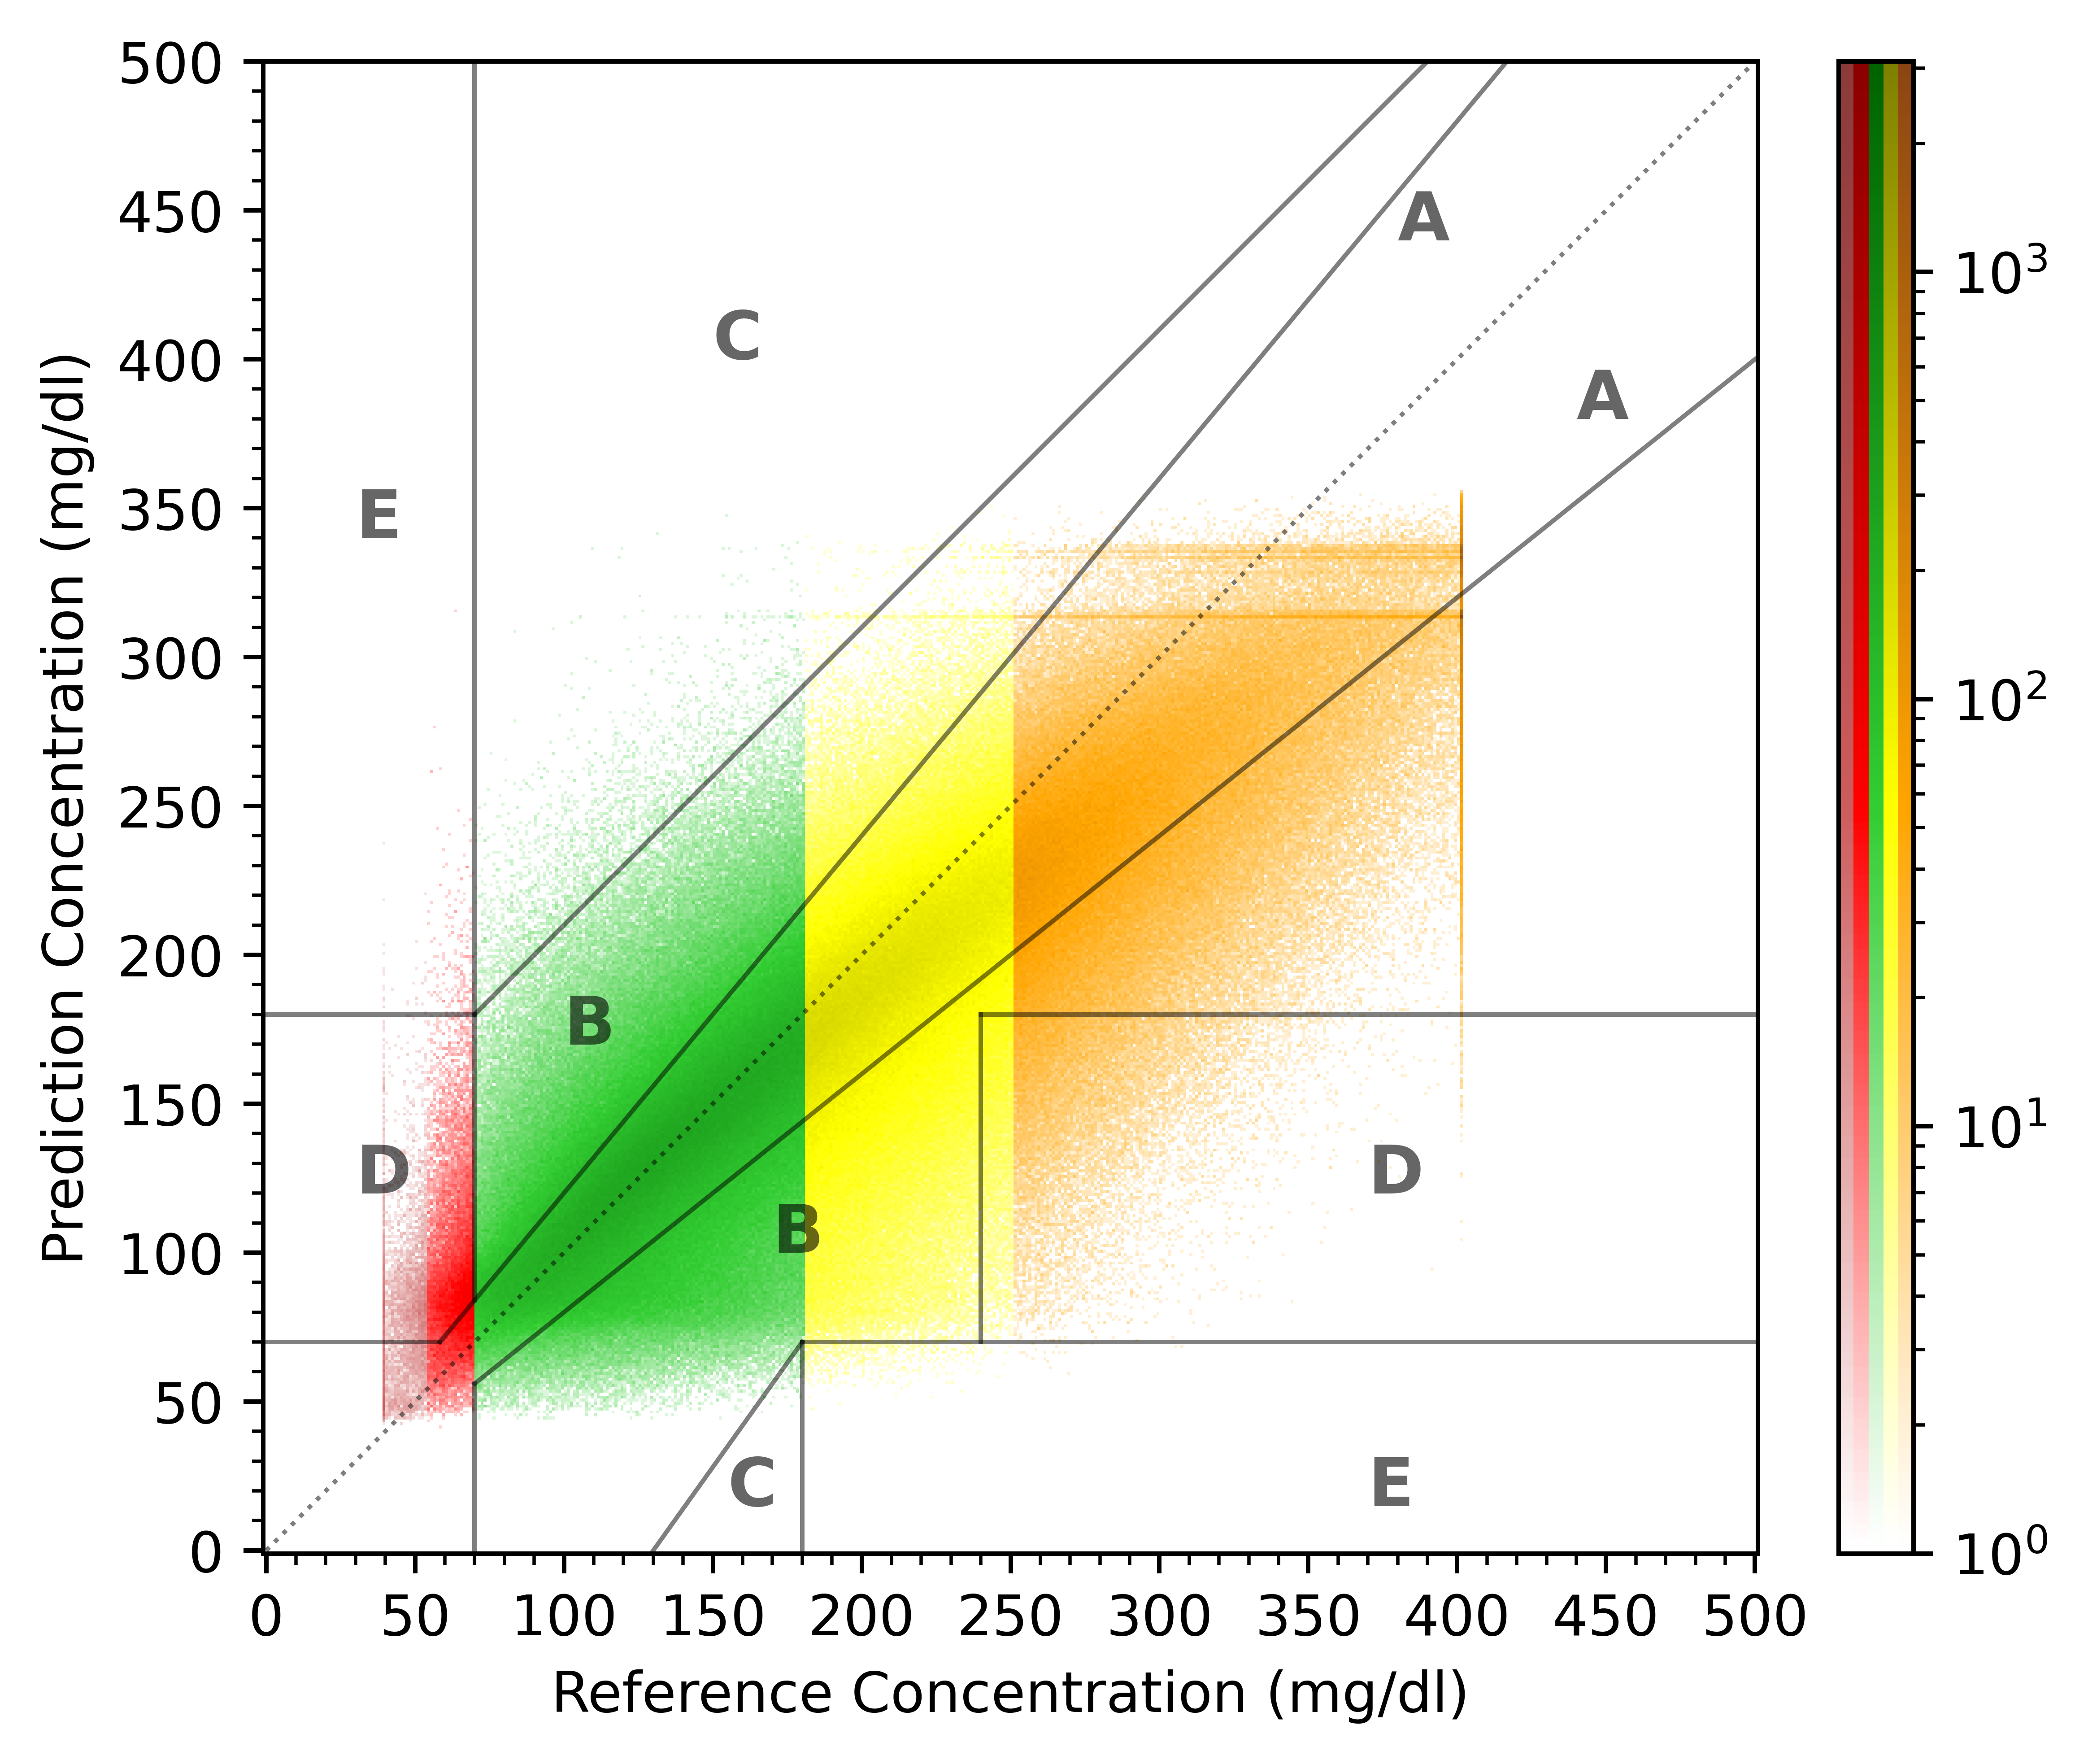
\includegraphics[width=0.82\textwidth]{images/CEGA_Diatrend/DiaTrend_random_semi.png}
    \caption{Clarke Error Grid for DiaTrend using random resampling and
    the semi-balanced target distribution.}
    \label{fig:diatrend_clarke_semi}
\end{figure}

\begin{figure}[htbp]
    \centering
    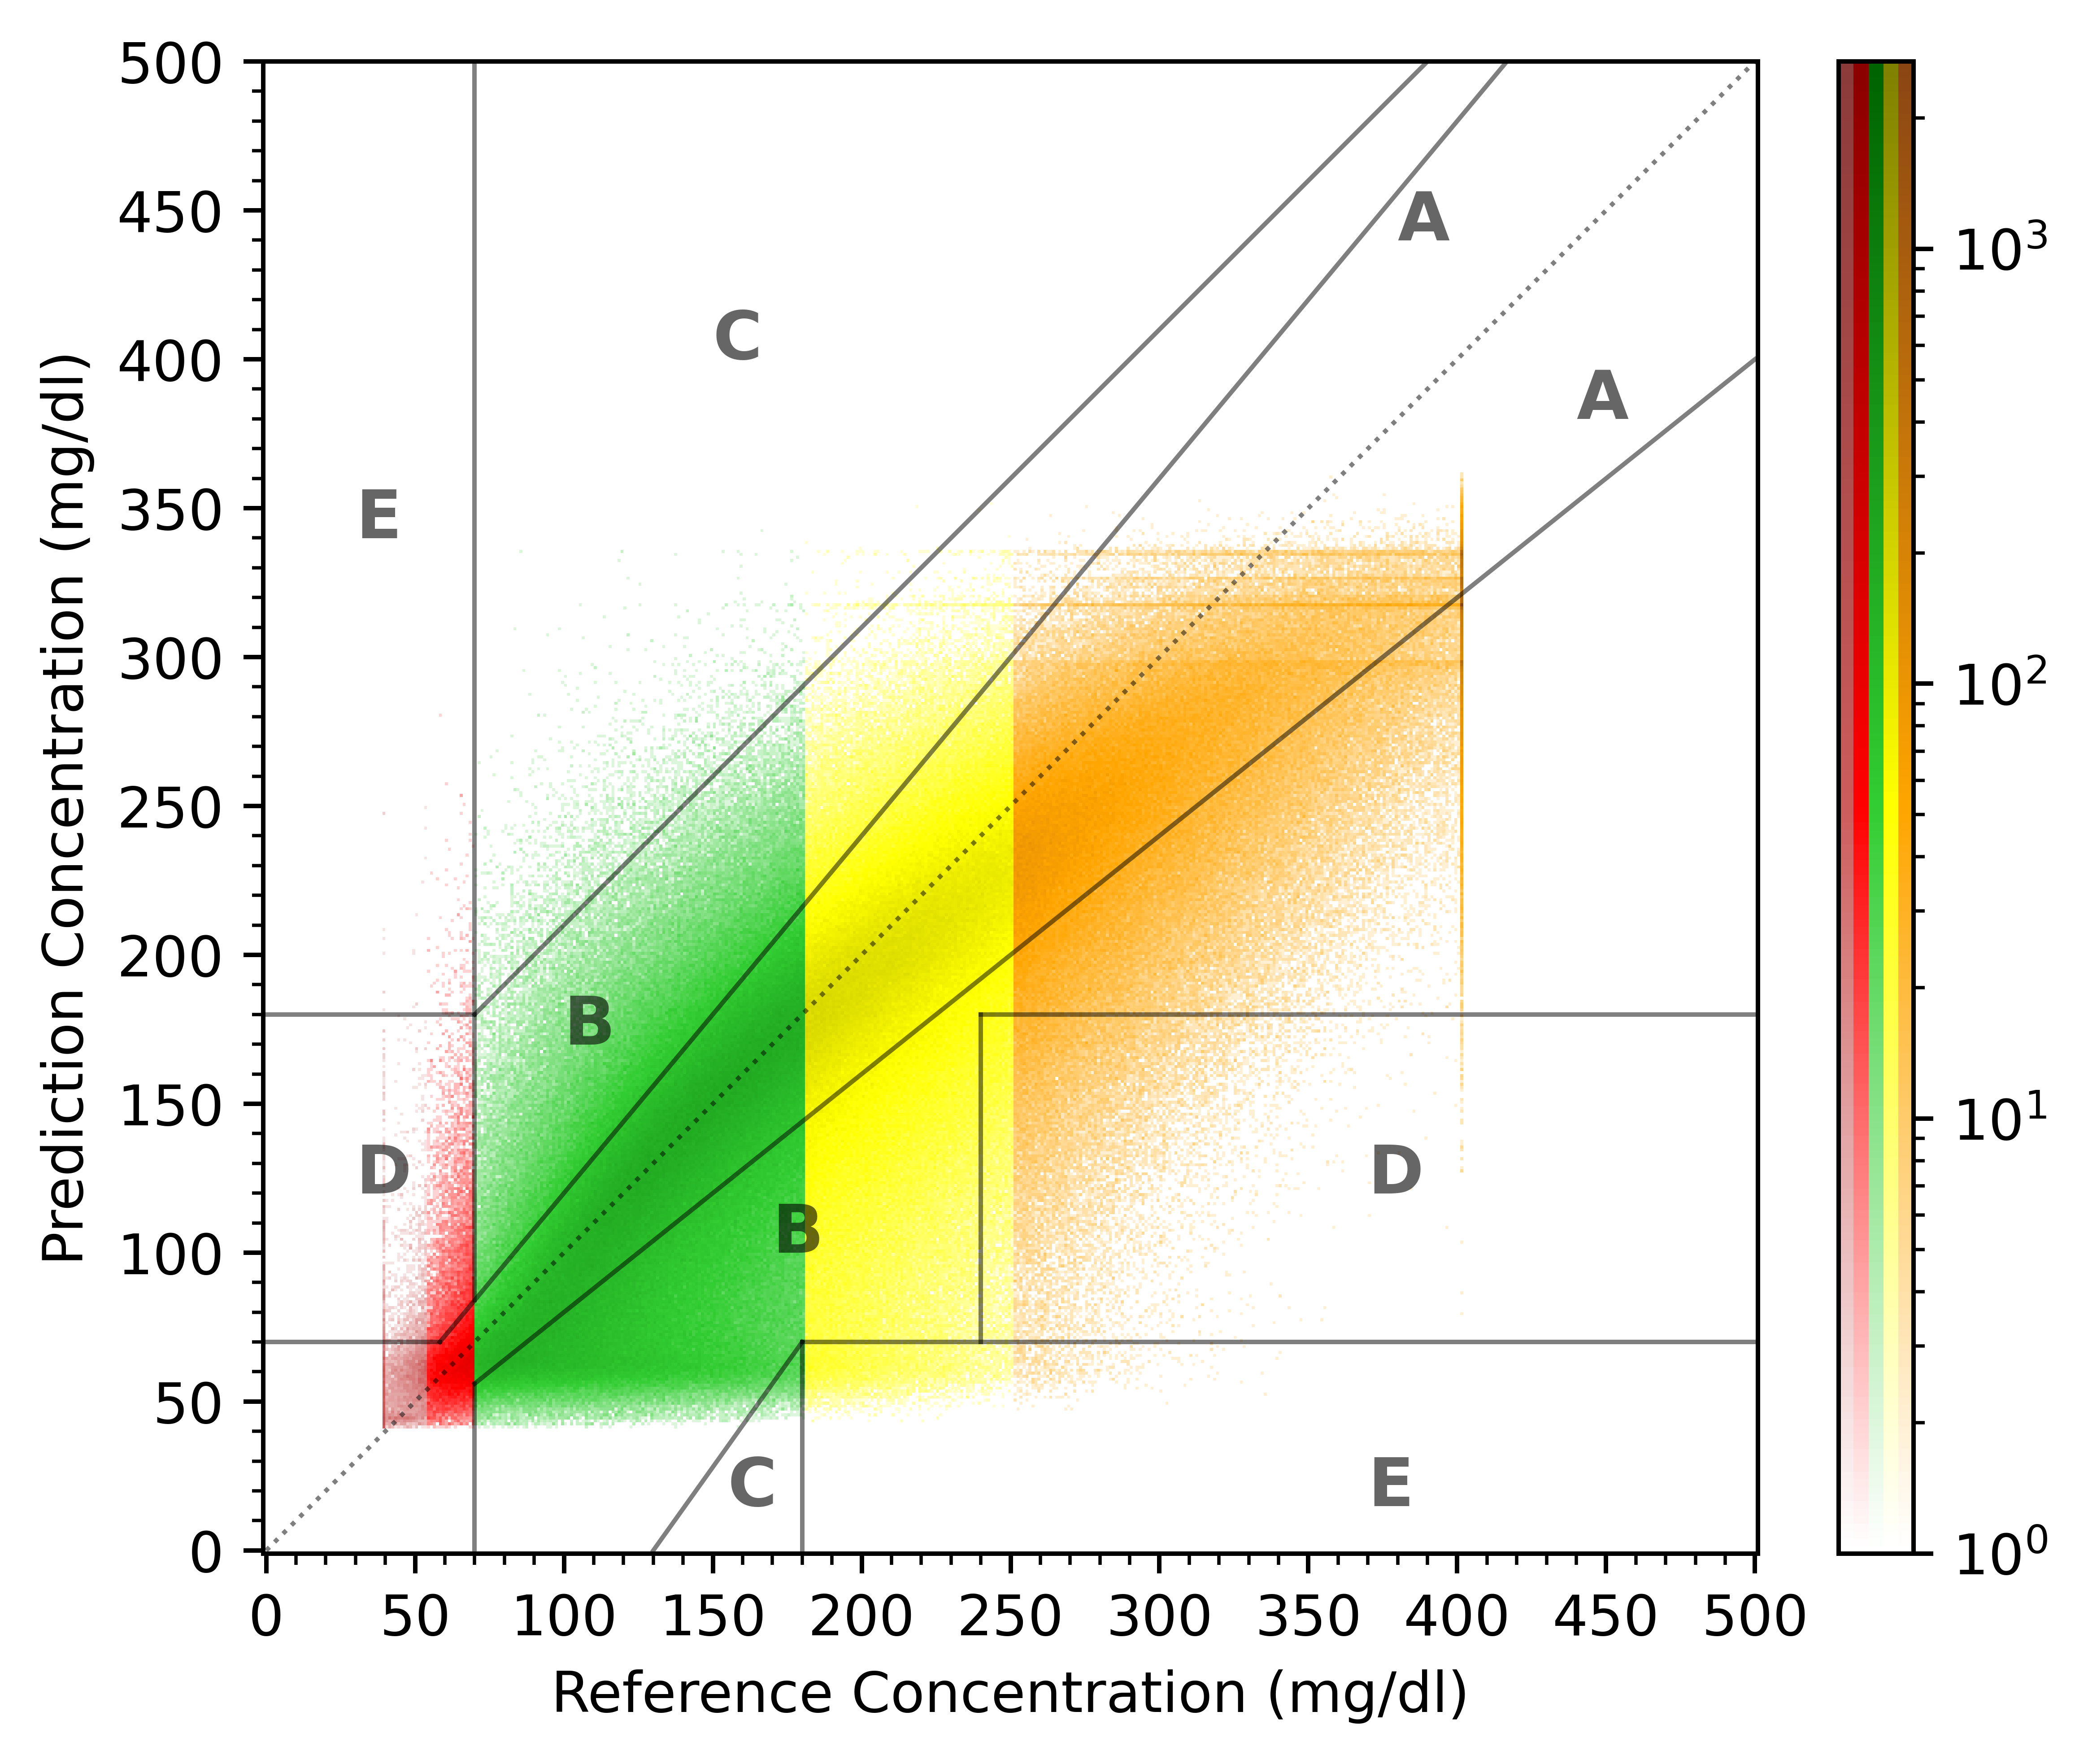
\includegraphics[width=0.82\textwidth]{images/CEGA_Diatrend/DiaTrend_random_full.png}
    \caption{Clarke Error Grid for DiaTrend using random resampling and
    the fully balanced target distribution.}
    \label{fig:diatrend_clarke_full}
\end{figure}

These Clarke Error Grids are consistent with the quantitative analysis. They support the interpretation that the increase in global RMSE under balancing does not represent a uniform clinical deterioration. Instead, it mainly reflects reduced numerical precision in TIR, together with a substantial improvement in hypoglycemia.

\subsection{DiaTrend Summary}
\label{subsec:diatrend_summary}

The primary statistical analysis rejected the null hypothesis for DiaTrend. Using the fold-level analysis, full balancing increased \(AB_{\mathrm{TBR_2}}\) by an average of \(63.75\) percentage points relative to the normalized baseline, with a one-sided \(p\)-value of \(0.00016\).

The aggregate secondary results support this conclusion. When predictions from all folds were combined, mean TBR$_2$ A+B across methods increased from \(3.74\%\) under normalized balancing to \(72.68\%\) under full balancing. TBR$_1$ A+B similarly increased from \(1.60\%\) to \(70.35\%\). These improvements were accompanied by substantial reductions in RMSE, MAE, and Zone D.

The balancing target was found to have a much greater influence on predictive behaviour than the selected resampling method. Random resampling, SMOTER, and SMOGN produced closely aligned aggregate results under the same target distribution, although formal equivalence between them was not tested.

Semi-balancing provided a favourable intermediate response. It substantially improved both hypoglycemic ranges while preserving global RMSE and producing only a limited deterioration in TIR numerical accuracy.

Overall, full balancing is considered the most beneficial DiaTrend configuration. The moderate deterioration in global and TIR numerical accuracy is definitely outweighed by the magnitude and clinical relevance of the improvements obtained in TBR.

% ============================================================
% REPLACE-BG
% ============================================================

\section{REPLACE-BG Results}
\label{sec:replacebg_results}

\begin{quote}
\small
\textit{Since the subsequent analyses for REPLACE-BG are analogous to the ones performed for Diatrend, some parts of the analysis methodology have been omitted.}
\end{quote}

\subsection{Primary Statistical Test}
\label{subsec:replacebg_primary_analysis}

The same statistical analysis defined in Section~\ref{sec:statistical_analysis} was also performed for REPLACE-BG. The resulting values are presented in Table~\ref{tab:replacebg_fold_primary_effect} and constitute the five observations used in the paired Student's \(t\)-test.

\begin{table}[htbp]
    \centering
    \caption{REPLACE-BG fold-level prediction performance for the primary clinical outcome.}
    \label{tab:replacebg_fold_primary_effect}
    \begin{tabular}{cccc}
        \toprule
        \textbf{Fold}
        & \textbf{Normalized A+B}
        & \textbf{Full A+B}
        & \(\boldsymbol{\Delta}\) \textbf{A+B} \\
        \midrule
        1 & 0.01\% & 78.97\% & +78.96 pp \\
        2 & 0.00\% & 78.62\% & +78.62 pp \\
        3 & 0.06\% & 76.98\% & +76.92 pp \\
        4 & 0.00\% & 76.00\% & +76.00 pp \\
        5 & 0.00\% & 73.54\% & +73.54 pp \\
        \midrule
        \textbf{Mean}
        & \textbf{0.01\%}
        & \textbf{76.82\%}
        & \textbf{+76.81 pp} \\
        \bottomrule
    \end{tabular}
\end{table}

Full balancing produced a positive improvement in every fold, with fold-level differences ranging from \(73.54\) to \(78.96\) percentage points. Additionally, all 15 individual method--fold comparisons were positive, with improvements ranging from \(72.72\) to \(80.08\) percentage points.

Therefore, the five observations used in the statistical test were:

\begin{equation}
d_f
\in
\{
78.96,\,
78.62,\,
76.92,\,
76.00,\,
73.54
\}
\text{ pp}.
\end{equation}

Their mean and standard deviation were:

\begin{equation}
\overline{d}
=
76.81
\text{ pp},
\end{equation}

\begin{equation}
s_d
=
2.20
\text{ pp}.
\end{equation}

Applying the one-sided paired Student's \(t\)-test produced the following statistic:

\begin{equation}
t
=
\frac{76.81}{2.20/\sqrt{5}}
=
78.23.
\end{equation}

With \(n-1=4\) degrees of freedom, the corresponding one-sided \(p\)-value was:

\begin{equation}
p
=
8.00 \times 10^{-8}.
\end{equation}

Since:

\begin{equation}
p < \alpha
\qquad
(8.00 \times 10^{-8} < 0.01),
\end{equation}

the null hypothesis defined in Equation~\ref{eq:null_hypothesis_tbr2} can be rejected for REPLACE-BG.

The statistical significance is also accompanied by a substantial and highly consistent effect magnitude. Mean \(AB_{\mathrm{TBR_2}}\) increased from approximately \(0.01\%\) under normalized balancing to \(76.82\%\) under full balancing. Therefore, the REPLACE-BG results support the primary study hypothesis and show an even more consistent fold-level effect than that observed for DiaTrend.

\subsection{Secondary Outcomes}
\label{subsec:replacebg_secondary_outcomes}

The secondary outcomes analysis follows the same procedure used for DiaTrend.

\subsubsection{Influence of the Balancing Method}
\label{subsubsec:replacebg_method_influence}

Table~\ref{tab:replacebg_method_influence} presents a condensed comparison of the principal global and hypoglycemic results.

\begin{table}[htbp]
    \centering
    \caption{Main REPLACE-BG results.}
    \label{tab:replacebg_method_influence}
    \resizebox{\textwidth}{!}{
    \begin{tabular}{lcccccc}
        \toprule
        \textbf{Target}
        & \textbf{Entire RMSE}
        & \textbf{Entire A+B}
        & \textbf{TBR$_2$ RMSE}
        & \textbf{TBR$_2$ A+B}
        & \textbf{TBR$_1$ RMSE}
        & \textbf{TBR$_1$ A+B} \\
        \midrule

        Normalized
        & \(36.48 \pm 0.12\)
        & \(95.08 \pm 0.02\)
        & \(56.99 \pm 0.47\)
        & \(0.01 \pm 0.02\)
        & \(41.89 \pm 0.43\)
        & \(0.33 \pm 0.20\) \\

        Semi-balanced
        & \(36.97 \pm 0.05\)
        & \(96.42 \pm 0.04\)
        & \(43.61 \pm 0.29\)
        & \(27.08 \pm 0.54\)
        & \(32.09 \pm 0.09\)
        & \(36.90 \pm 1.05\) \\

        Fully balanced
        & \(41.18 \pm 0.05\)
        & \(97.55 \pm 0.04\)
        & \(32.57 \pm 0.72\)
        & \(76.89 \pm 0.85\)
        & \(24.92 \pm 0.46\)
        & \(78.49 \pm 0.65\) \\

        \bottomrule
    \end{tabular}
    }
\end{table}

As in DiaTrend, the differences between balancing methods were small compared with the changes introduced by the target distribution. The standard deviation of global RMSE remained at or below \(0.12\) mg/dL, while the standard deviation of global A+B remained below \(0.05\) percentage points, for both semi and full balancing targets distributions.

Therefore -- although formal equivalence between methods is not demonstrated -- the REPLACE-BG results also support the idea that balancing intensity has a much greater influence on predictive performance than any particular resampling method.

\subsubsection{Effect of Balancing Intensity in Hypoglycemia}
\label{subsubsec:replacebg_semi_balancing}

Table~\ref{tab:replacebg_hypoglycemia} presents the aggregate results for TBR$_2$ and TBR$_1$. As in DiaTrend.

\begin{table}[htbp]
    \centering
    \caption{REPLACE-BG performance in the hypoglycemic ranges,
    averaged across balancing methods.}
    \label{tab:replacebg_hypoglycemia}
    \resizebox{\textwidth}{!}{
    \begin{tabular}{llccccc}
        \toprule
        \textbf{Target}
        & \textbf{Range}
        & \textbf{RMSE}
        & \textbf{MAE}
        & \textbf{A+B}
        & \textbf{Zone D}
        & \textbf{Zone E} \\
        \midrule

        Normalized & TBR$_2$
        & 56.99 & 53.96 & 0.01\% & 99.29\% & 0.69\% \\

        Semi-balanced & TBR$_2$
        & 43.61 & 36.13 & \textbf{27.08\%} & 72.08\% & 0.84\% \\

        Fully balanced & TBR$_2$
        & \textbf{32.57} & 20.69 & \textbf{76.89\%} & 22.22\% & 0.88\% \\

        \midrule

        Normalized & TBR$_1$
        & 41.89 & 38.18 & 0.33\% & 99.05\% & 0.62\% \\

        Semi-balanced & TBR$_1$
        & 32.09 & 23.27 & \textbf{36.90\%} & 62.32\% & 0.78\% \\

        Fully balanced & TBR$_1$
        & \textbf{24.92} & 13.49 & \textbf{78.49\%} & 20.69\% & 0.82\% \\

        \bottomrule
    \end{tabular}
    }
\end{table}

Semi-balancing produced substantial improvements. Relative to the normalized baseline, TBR$_2$ RMSE decreased by \(13.38\) mg/dL and A+B increased by \(27.06\) percentage points. In TBR$_1$, RMSE decreased by \(9.80\) mg/dL and A+B increased by \(36.56\) percentage points.

Like in Diatrend analysis, full balancing intensified this effect. TBR$_2$ RMSE decreased by \(24.42\) mg/dL, while A+B increased by \(76.88\) percentage points. TBR$_1$ RMSE decreased by \(16.97\) mg/dL, and A+B increased by \(78.16\) percentage points. Once more, the clinical improvements were mainly produced by a movement from Zone D into Zone A.

The results therefore show the same descriptive relationship between balancing intensity in hypoglycemic performance, described by Equation~\ref{eq:ordered_hypothesis_conjecture}

\subsubsection{Global and Time-in-Range Trade-Off}
\label{subsubsec:replacebg_global_tir}

Table~\ref{tab:replacebg_global_tir} summarizes global and TIR performance after balancing the training sets.

\begin{table}[htbp]
    \centering
    \caption{Aggregate global and TIR performance in REPLACE-BG,
    averaged across balancing methods.}
    \label{tab:replacebg_global_tir}
    \resizebox{\textwidth}{!}{
    \begin{tabular}{llccccc}
        \toprule
        \textbf{Target}
        & \textbf{Range}
        & \textbf{RMSE}
        & \textbf{MAE}
        & \textbf{A+B}
        & \textbf{Zone D}
        & \textbf{Zone E} \\
        \midrule

        Normalized & Entire
        & 36.48 & 26.71 & 95.08\% & 4.75\% & 0.02\% \\

        Semi-balanced & Entire
        & 36.97 & 26.57 & 96.42\% & 3.29\% & 0.08\% \\

        Fully balanced & Entire
        & \textbf{41.18} & 30.11 & \textbf{97.55\%} & 1.66\% & 0.44\% \\

        \midrule

        Normalized & TIR
        & 26.27 & 19.36 & 99.80\% & \textbf{0.00\%} & \textbf{0.00\%} \\

        Semi-balanced & TIR
        & 29.57 & 21.30 & 99.71\% & \textbf{0.00\%} & \textbf{0.00\%} \\

        Fully balanced & TIR
        & \textbf{35.89} & 27.05 & 99.46\% & \textbf{0.00\%} & \textbf{0.00\%} \\

        \bottomrule
    \end{tabular}
    }
\end{table}

Semi-balancing increased global RMSE by only \(0.49\) mg/dL and reduced MAE by \(0.15\) mg/dL. At the same time, global A+B increased by \(1.34\) percentage points and Zone D decreased by \(1.46\) percentage points.

In TIR, semi-balancing increased RMSE by \(3.30\) mg/dL, but A+B decreased by only \(0.09\) percentage points and remained at \(99.71\%\). The impact is also infimal.

Full balancing produced a larger numerical deterioration. Global RMSE increased by \(4.70\) mg/dL and MAE by \(3.39\) mg/dL. Nevertheless, global A+B increased by \(2.47\) percentage points, while Zone D decreased
from \(4.75\%\) to \(1.66\%\).

In this case, the largest numerical cost also appeared in TIR when full balancing, where RMSE increased by \(9.62\) mg/dL. However, TIR A+B decreased by only \(0.34\) percentage points and remained at \(99.46\%\). No TIR predictions were located in Zones D or E.

Therefore, as in DiaTrend, the deterioration in TIR was mainly numerical rather than clinical. The global RMSE increase is strongly influenced by the reduced numerical precision in TIR, while global clinical acceptability actually improved slightly.

\subsubsection{Hyperglycemic-Range Performance}
\label{subsubsec:replacebg_hyperglycemia}

Table~\ref{tab:replacebg_hyperglycemia} presents the results for moderate and severe hyperglycemia.

\begin{table}[htbp]
    \centering
    \caption{Aggregate REPLACE-BG performance in the hyperglycemic
    ranges, averaged across balancing methods.}
    \label{tab:replacebg_hyperglycemia}
    \resizebox{\textwidth}{!}{
    \begin{tabular}{llccccc}
        \toprule
        \textbf{Target}
        & \textbf{Range}
        & \textbf{RMSE}
        & \textbf{MAE}
        & \textbf{A+B}
        & \textbf{Zone D}
        & \textbf{Zone E} \\
        \midrule

        Normalized & TAR$_1$
        & 42.35 & 33.35 & 98.29\% & 1.66\% & 0.00\% \\

        Semi-balanced & TAR$_1$
        & 42.26 & 31.74 & 98.37\% & 1.37\% & 0.20\% \\

        Fully balanced & TAR$_1$
        & 46.21 & 33.30 & 97.04\% & 1.29\% & \textbf{1.62\%} \\

        \midrule

        Normalized & TAR$_2$
        & 65.80 & 55.27 & 91.62\% & 8.38\% & 0.00\% \\

        Semi-balanced & TAR$_2$
        & 61.65 & 50.37 & 93.13\% & 6.83\% & 0.03\% \\

        Fully balanced & TAR$_2$
        & \textbf{61.76} & 49.36 & \textbf{93.21\%} & 6.50\% & 0.29\% \\

        \bottomrule
    \end{tabular}
    }
\end{table}

Semi-balancing slightly improved TAR$_1$: RMSE decreased by \(0.09\) mg/dL, MAE by \(1.61\) mg/dL, and A+B increased by \(0.08\) percentage points. The improvement was clearer in TAR$_2$, where RMSE decreased by \(4.15\) mg/dL and A+B increased by \(1.51\) percentage points.

Full balancing maintained the TAR$_2$ improvement. Relative to normalized balancing, RMSE decreased by \(4.04\) mg/dL, MAE by \(5.91\) mg/dL, and A+B increased by \(1.59\) percentage points.

In contrast, TAR$_1$ showed a localized deterioration under full balancing. RMSE increased by \(3.86\) mg/dL and A+B decreased by \(1.25\) percentage points. Zone E also increased from zero to \(1.62\%\).

This pattern is closely aligned with DiaTrend: severe hyperglycemia also benefited from balancing, whereas full balancing introduced a smaller adverse effect in moderate hyperglycemia.

\subsubsection{Clarke Error Grid Interpretation}
\label{subsubsec:replacebg_clarke_interpretation}

Figures~\ref{fig:replacebg_clarke_normalized}, \ref{fig:replacebg_clarke_semi}, and \ref{fig:replacebg_clarke_full} present representative Clarke Error Grids for the normalized baseline, semi-balanced, and fully balanced random-resampling configurations, respectively.

\begin{figure}[htbp]
    \centering
    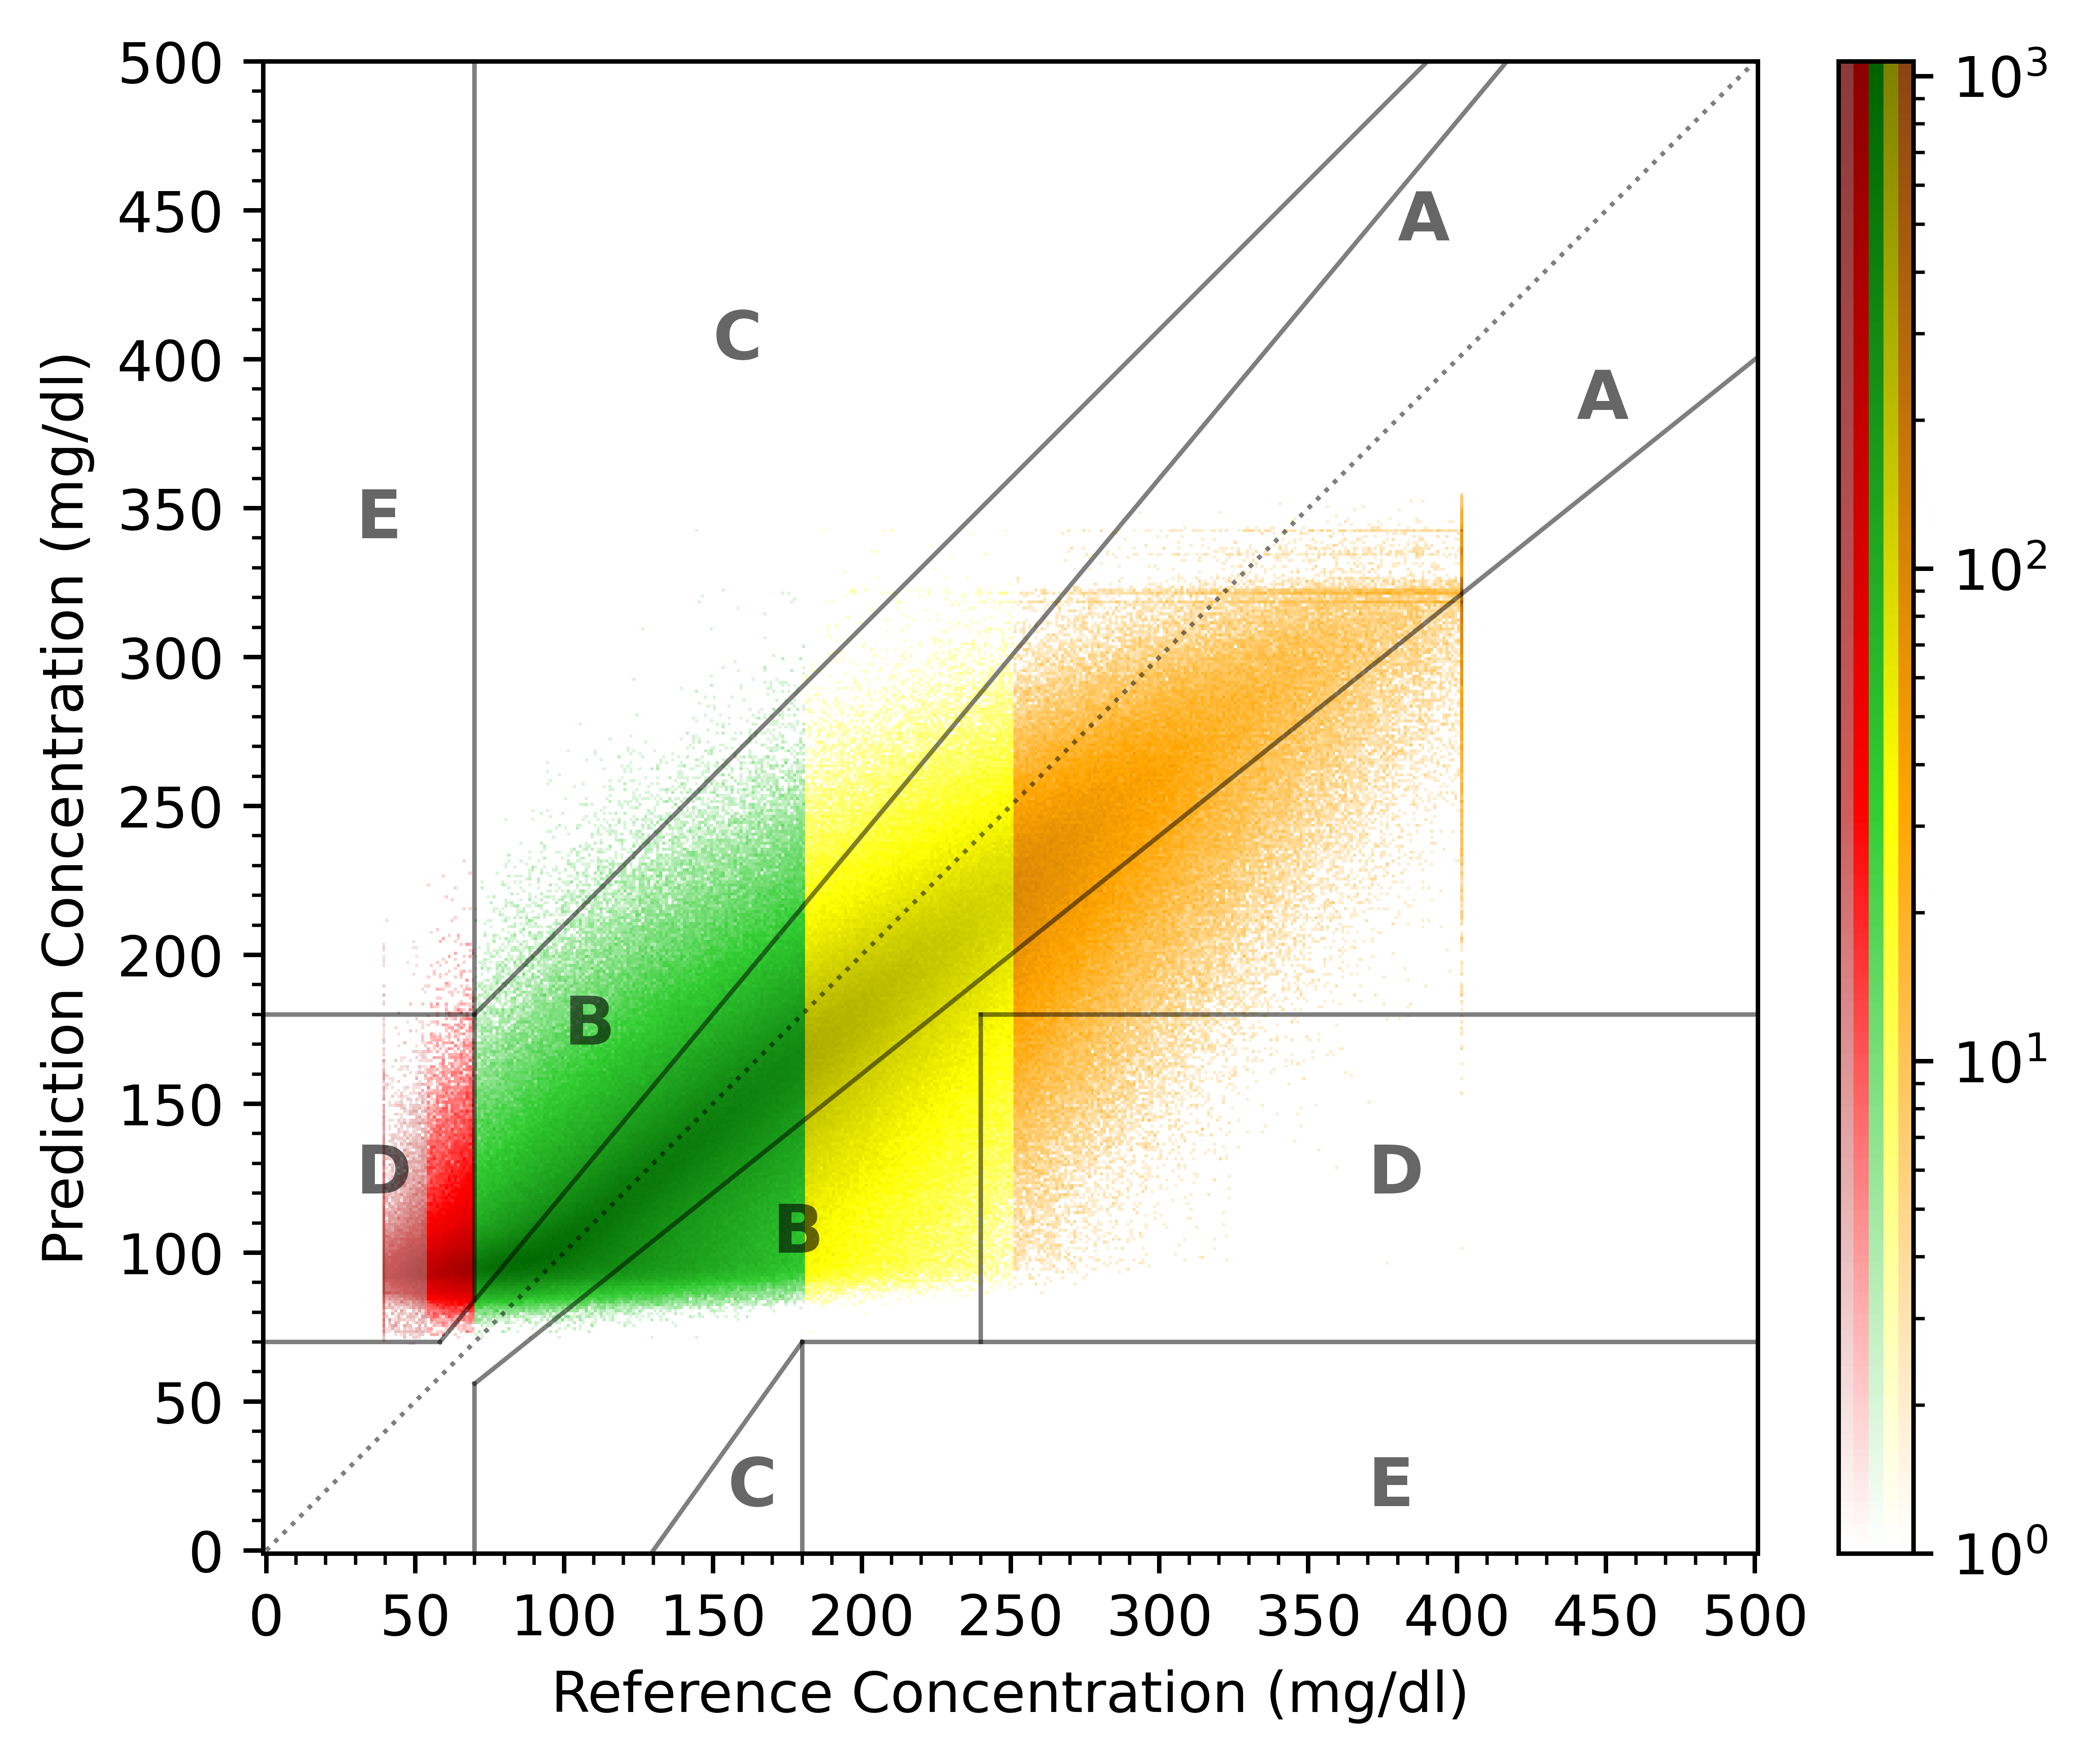
\includegraphics[width=0.82\textwidth]
    {images/CEGA_REPLACE-BG/REPLACE-BG_random_normalized.png}
    \caption{Clarke Error Grid for REPLACE-BG using random resampling and
    the normalized baseline target distribution.}
    \label{fig:replacebg_clarke_normalized}
\end{figure}

\begin{figure}[htbp]
    \centering
    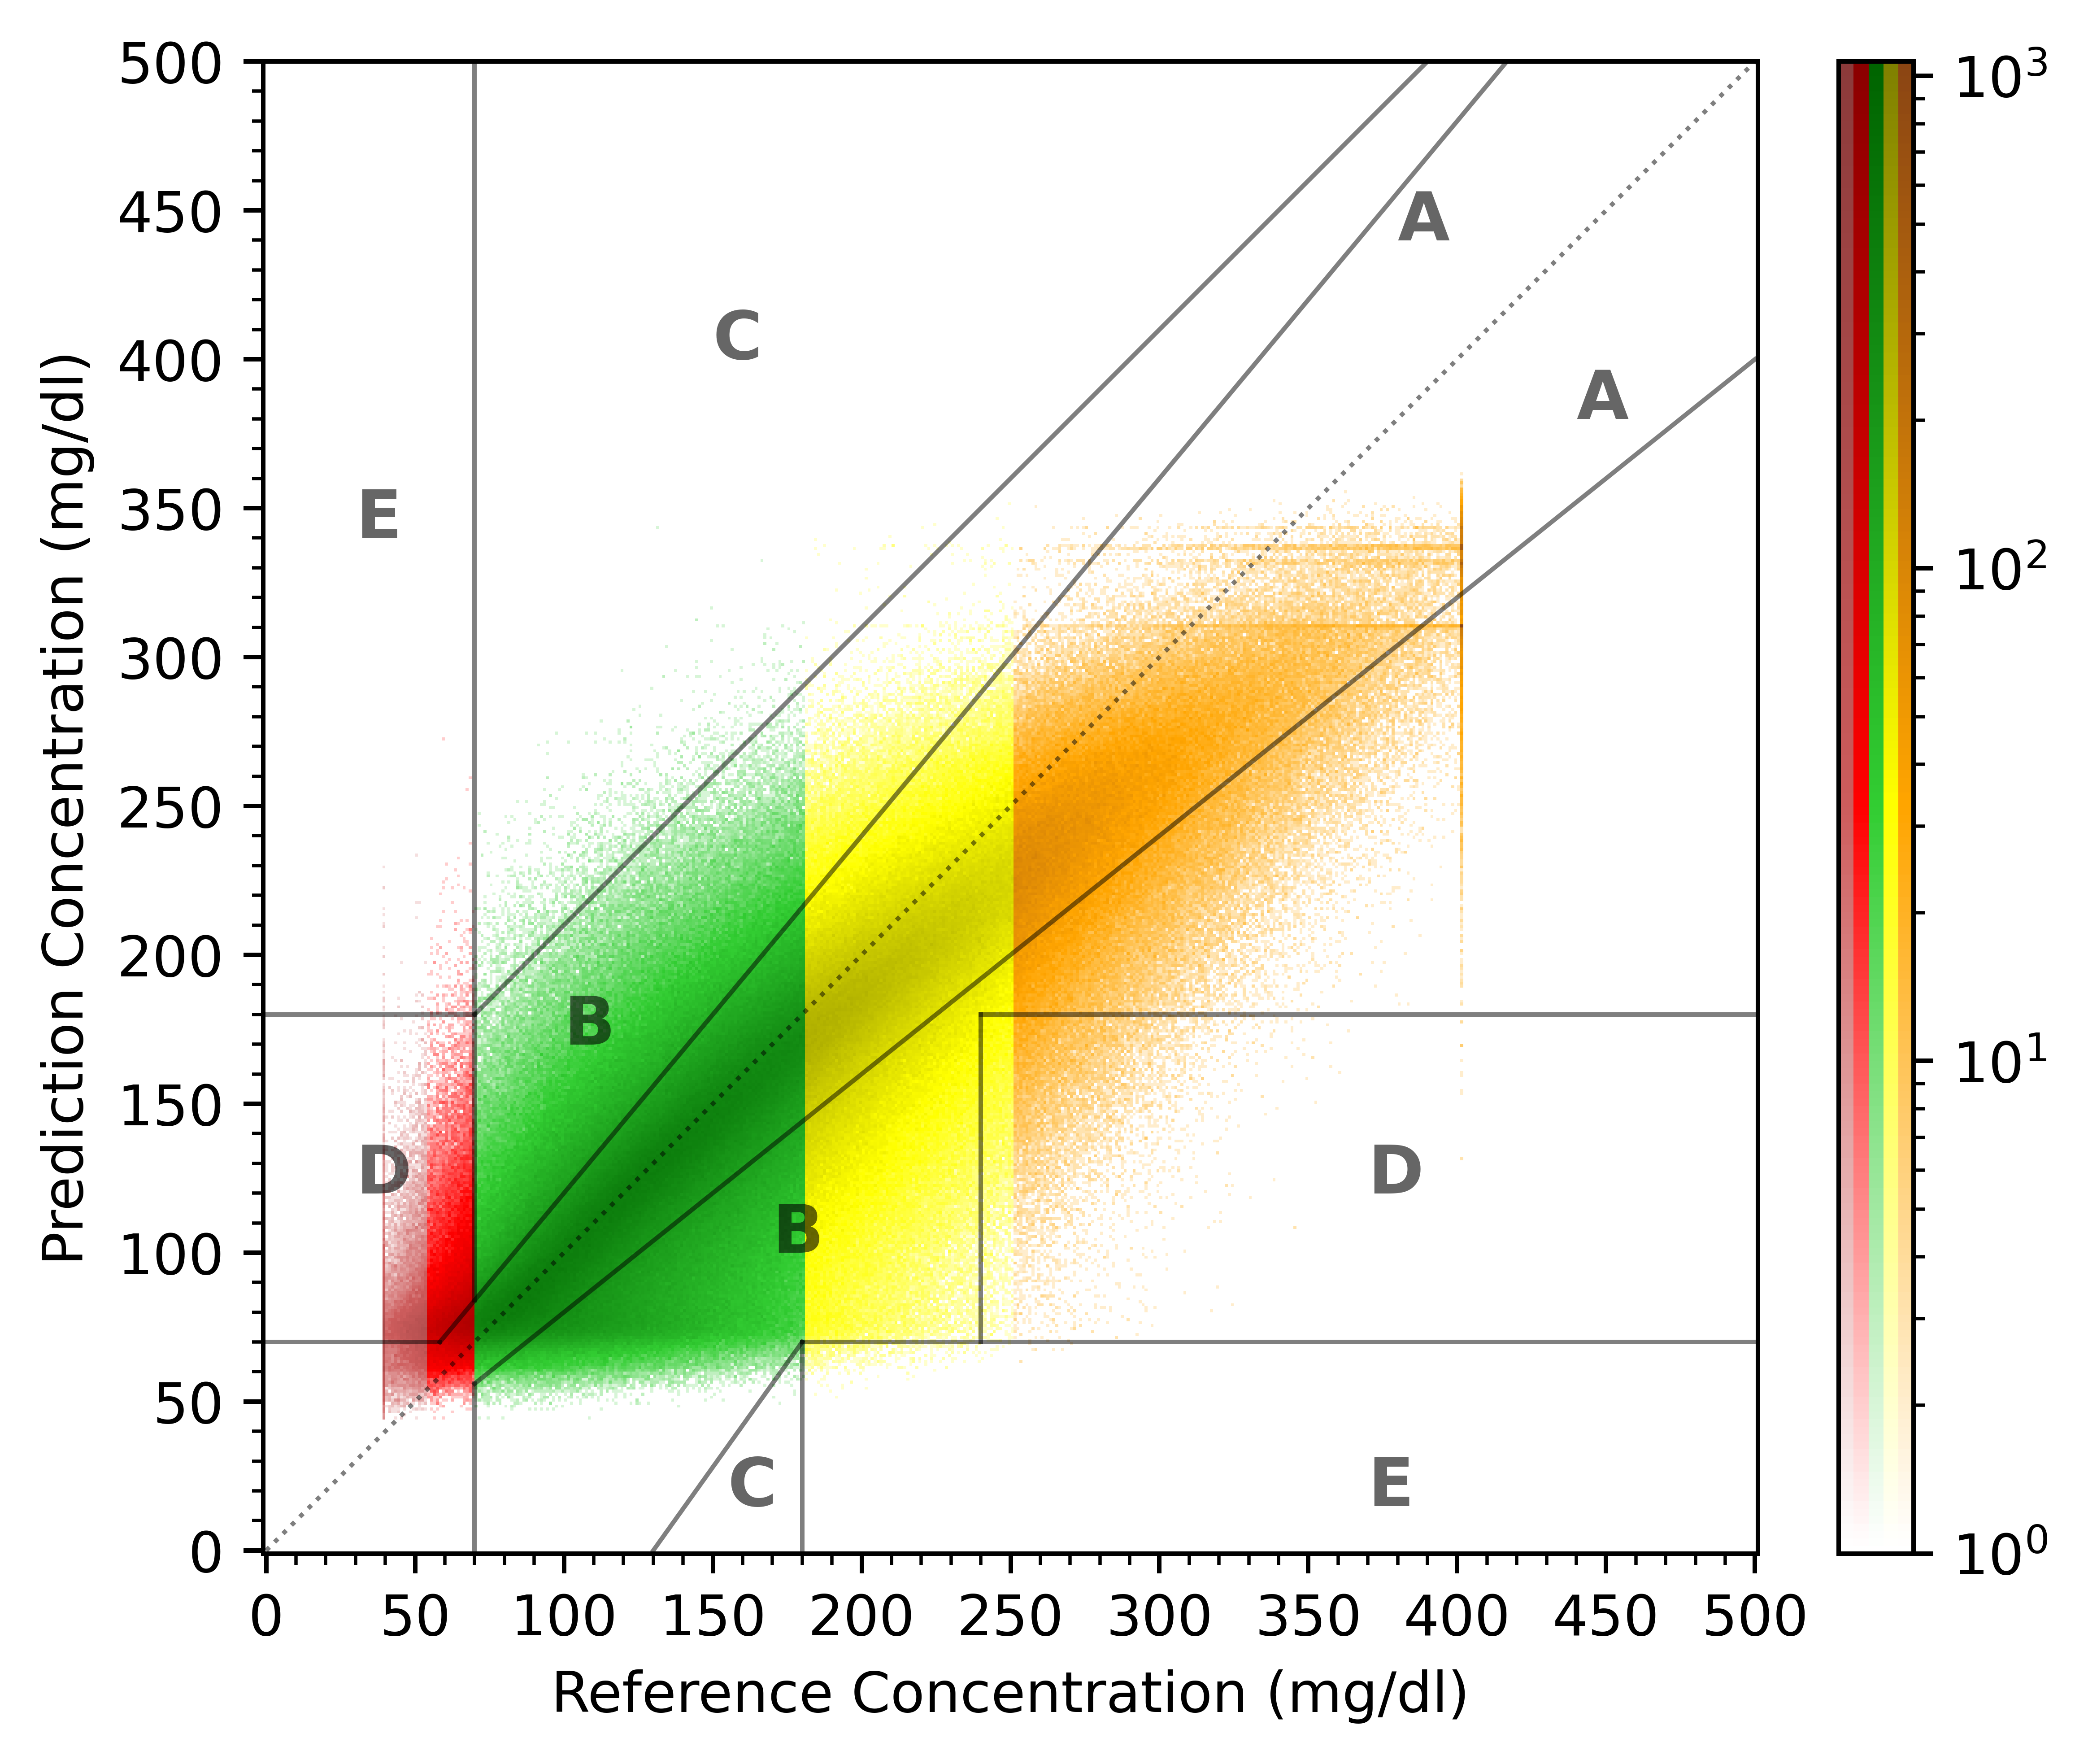
\includegraphics[width=0.82\textwidth]
    {images/CEGA_REPLACE-BG/REPLACE-BG_random_semi.png}
    \caption{Clarke Error Grid for REPLACE-BG using random resampling and
    the semi-balanced target distribution.}
    \label{fig:replacebg_clarke_semi}
\end{figure}

\begin{figure}[htbp]
    \centering
    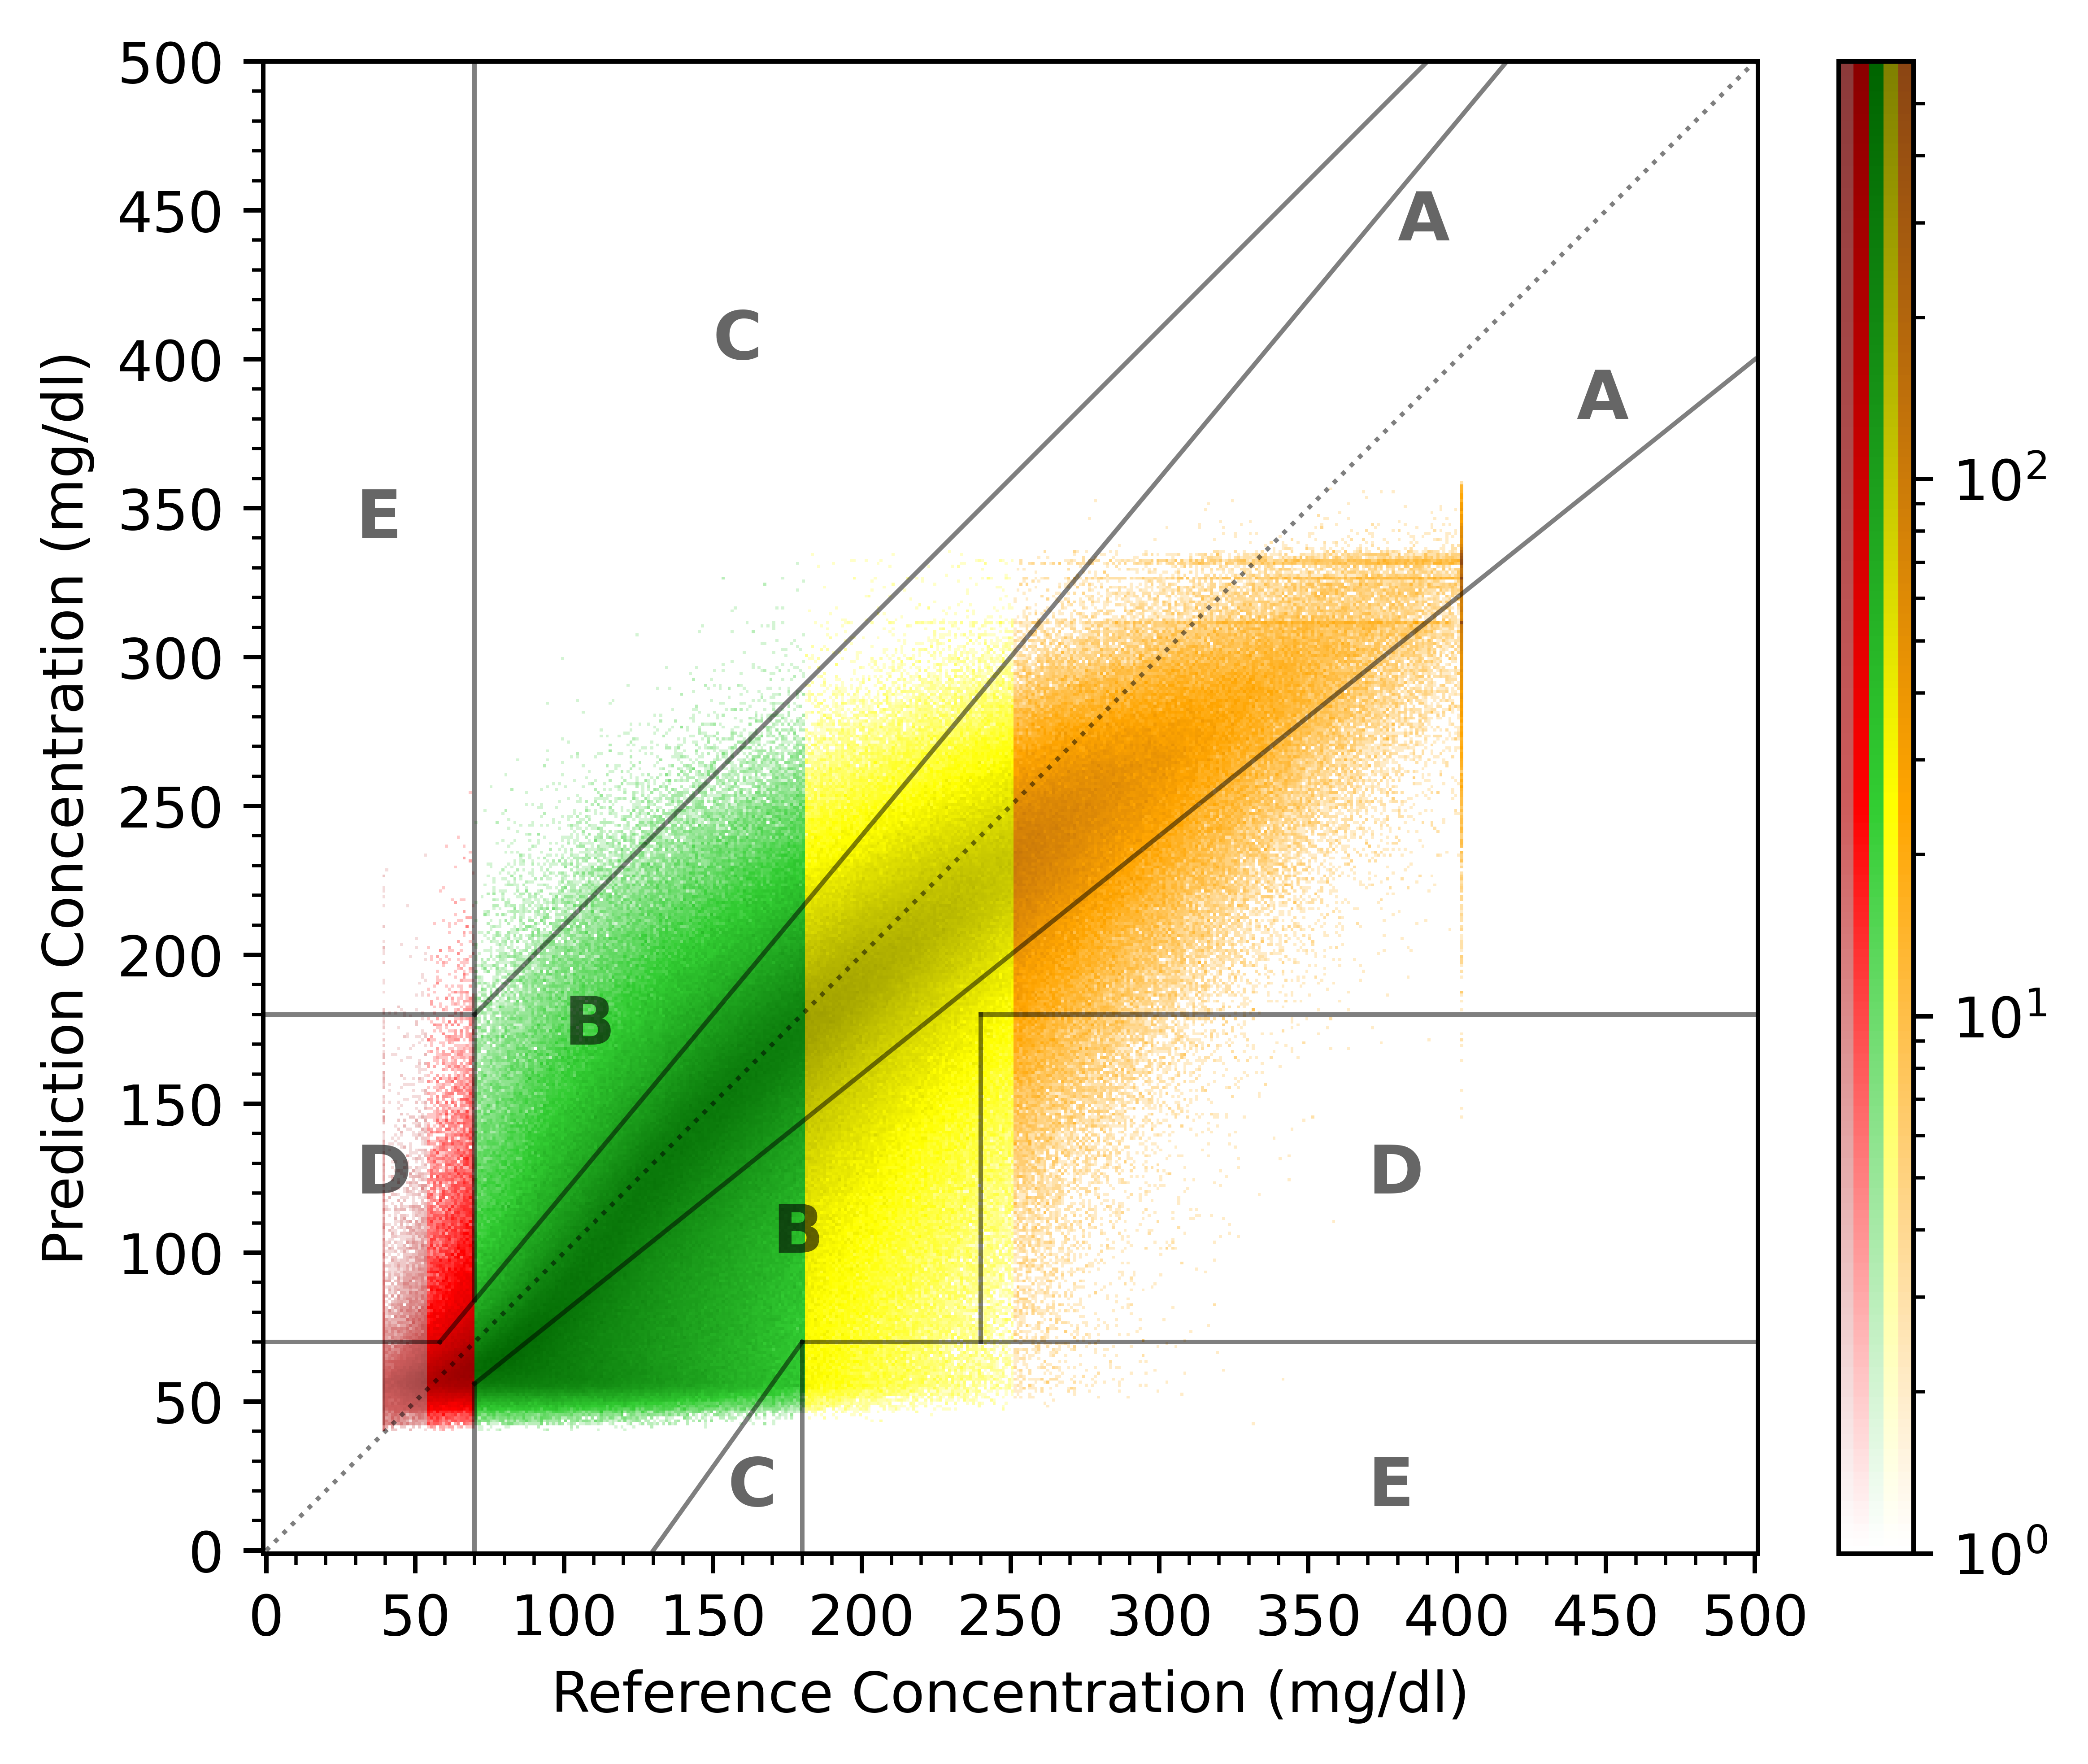
\includegraphics[width=0.82\textwidth]
    {images/CEGA_REPLACE-BG/REPLACE-BG_random_full.png}
    \caption{Clarke Error Grid for REPLACE-BG using random resampling and
    the fully balanced target distribution.}
    \label{fig:replacebg_clarke_full}
\end{figure}

The grids support the range-specific results. Increasing the balancing
intensity produces a substantial movement of hypoglycemic predictions from
Zone D into Zone A. At the same time, the wider dispersion in the central
glucose region is consistent with the increase in TIR RMSE.

As in DiaTrend, the increase in global numerical error therefore does not
represent a uniform deterioration across the complete glucose spectrum. It is
mainly associated with reduced numerical precision in TIR, together with a
major improvement in the clinically critical hypoglycemic regions.

\subsection{REPLACE-BG Summary}
\label{subsec:replacebg_summary}

The primary statistical analysis rejected the null hypothesis for REPLACE-BG with a one-sided \(p\)-value of \(8.00 \times 10^{-8}\). The improvement was also positive in every fold and in all 15 method--fold comparisons.

The aggregate results support this conclusion. Mean TBR$_2$ A+B increased from \(0.01\%\) under normalized balancing to \(76.89\%\) under full balancing, while TBR$_1$ A+B increased from \(0.33\%\) to \(78.49\%\). These improvements were accompanied by substantial reductions in RMSE,
MAE, and Zone D.

The balancing target again had a much greater influence than the selected resampling method. Semi-balancing provided an effective intermediate configuration.

Full balancing produced the strongest improvements in TBR$_2$ and TBR$_1$. Its main cost was reduced numerical precision in TIR, although TIR A+B remained above \(99\%\) and no predictions entered Zones D or E. Severe hyperglycemia also improved, while moderate hyperglycemia presented a smaller localized deterioration.

Overall, full balancing is considered the most beneficial REPLACE-BG configuration. Its increase in global and TIR numerical error is considerably outweighed by the magnitude, consistency, and clinical relevance of the improvements in the hypoglycemic ranges.

% ============================================================
% T1DIABETESGRANADA
% ============================================================

\section{T1DiabetesGranada Results}
\label{sec:t1diabetesgranadaresults}

\begin{quote}
\small
\textit{Part of the analysis methodology has been omitted since it is analogus to the one performed for both Diatrend and REPLACE-BG. Some results are presented and discussed directly}.
\end{quote}

\subsection{Primary Statistical Test}
\label{subsec:t1diabetesgranadaprimary_analysis}

Table~\ref{tab:t1diabetesgranada_fold_primary_effect} presents the resulting five fold-level observations arise from the primary statistical analysis.

\begin{table}[htbp]
    \centering
    \caption{T1DiabetesGranada fold-level prediction performance for the primary clinical outcome.}
    \label{tab:t1diabetesgranada_fold_primary_effect}
    \begin{tabular}{cccc}
        \toprule
        \textbf{Fold}
        & \textbf{Normalized A+B}
        & \textbf{Full A+B}
        & \(\boldsymbol{\Delta}\) \textbf{A+B} \\
        \midrule
        1 & 12.46\% & 88.85\% & +76.39 pp \\
        2 & 12.18\% & 89.32\% & +77.14 pp \\
        3 & 5.98\%  & 90.16\% & +84.18 pp \\
        4 & 16.21\% & 88.61\% & +72.40 pp \\
        5 & 18.17\% & 87.69\% & +69.53 pp \\
        \midrule
        \textbf{Mean}
        & \textbf{13.00\%}
        & \textbf{88.93\%}
        & \textbf{+75.93 pp} \\
        \bottomrule
    \end{tabular}
\end{table}

Full balancing produced a positive improvement in every fold, with fold-level differences ranging from \(69.53\) to \(84.18\) percentage points. All 15 individual method--fold comparisons were also positive, with improvements ranging from \(67.60\) to \(90.53\) percentage points.

The five observations used in the statistical test were:

\begin{equation}
d_f
\in
\{
76.39,\,
77.14,\,
84.18,\,
72.40,\,
69.53
\}
\text{ pp}.
\end{equation}

Their mean and standard deviation were:

\begin{equation}
\overline{d}
=
75.93
\text{ pp},
\end{equation}

\begin{equation}
s_d
=
5.55
\text{ pp}.
\end{equation}

Applying the one-sided paired Student's \(t\)-test produced the following statistic:

\begin{equation}
t
=
\frac{75.93}{5.55/\sqrt{5}}
=
30.60.
\end{equation}

With \(n-1=4\) degrees of freedom, the corresponding one-sided
\(p\)-value was:

\begin{equation}
p
=
3.40 \times 10^{-6}.
\end{equation}

Since:

\begin{equation}
p < \alpha
\qquad
(3.40 \times 10^{-6} < 0.01),
\end{equation}

the null hypothesis defined in Equation~\ref{eq:null_hypothesis_tbr2} can definitely be rejected for T1DiabetesGranada.

Full balancing increased mean \(AB_{\mathrm{TBR_2}}\) from \(13.00\%\) to \(88.93\%\), corresponding to an average improvement of \(75.93\) percentage points. The magnitude and consistency of this effect support the primary study hypothesis for T1DiabetesGranada.

\subsection{Secondary Outcomes}
\label{subsec:t1diabetesgranadasecondary_outcomes}

Apart from the primar statistical test, an additional numerical analysis was performed on different secondary outcomes also for T1DiabetesGranada.

\subsubsection{Influence of the Balancing Method}
\label{subsubsec:t1diabetesgranadamethod_influence}

Table~\ref{tab:t1diabetesgranada_method_influence} summarizes the main global and hypoglycemic outcomes.

\begin{table}[htbp]
    \centering
    \caption{Main T1DiabetesGranada results.}
    \label{tab:t1diabetesgranada_method_influence}
    \resizebox{\textwidth}{!}{
    \begin{tabular}{lcccccc}
        \toprule
        \textbf{Target}
        & \textbf{Entire RMSE}
        & \textbf{Entire A+B}
        & \textbf{TBR$_2$ RMSE}
        & \textbf{TBR$_2$ A+B}
        & \textbf{TBR$_1$ RMSE}
        & \textbf{TBR$_1$ A+B} \\
        \midrule

        Normalized
        & \(37.80 \pm 0.00\)
        & \(94.26 \pm 0.04\)
        & \(40.83 \pm 0.28\)
        & \(13.24 \pm 1.07\)
        & \(36.82 \pm 0.29\)
        & \(8.47 \pm 1.07\) \\

        Semi-balanced
        & \(37.68 \pm 0.07\)
        & \(96.45 \pm 0.03\)
        & \(28.32 \pm 0.25\)
        & \(66.96 \pm 0.79\)
        & \(29.40 \pm 0.15\)
        & \(50.53 \pm 0.50\) \\

        Fully balanced
        & \(40.10 \pm 0.21\)
        & \(97.53 \pm 0.02\)
        & \(21.70 \pm 0.26\)
        & \(88.87 \pm 0.41\)
        & \(24.46 \pm 0.17\)
        & \(79.06 \pm 0.49\) \\

        \bottomrule
    \end{tabular}
    }
\end{table}

The variability across methods was again small relative to the differences between balancing targets. The standard deviation of global A+B remained below \(0.05\) percentage points, while the standard deviation of global RMSE did not exceed \(0.21\) mg/dL.

Under full balancing, aggregate TBR$_2$ A+B ranged from \(88.30\%\) to \(89.25\%\), while TBR$_1$ A+B ranged from \(78.47\%\) to \(79.66\%\). Therefore -- although formal equivalence was not tested -- the results again suggest that predictive performance depends mainly on balancing intensity rather than on the particular resampling method.

\subsubsection{Effect of Balancing Intensity in Hypoglycemia}
\label{subsubsec:t1diabetesgranadasemi_balancing}

Table~\ref{tab:t1diabetesgranada_hypoglycemia} presents the aggregate results for TBR$_2$ and TBR$_1$.

\begin{table}[htbp]
    \centering
    \caption{T1DiabetesGranada performance in the hypoglycemic ranges,
    averaged across balancing methods.}
    \label{tab:t1diabetesgranada_hypoglycemia}
    \resizebox{\textwidth}{!}{
    \begin{tabular}{llccccc}
        \toprule
        \textbf{Target}
        & \textbf{Range}
        & \textbf{RMSE}
        & \textbf{MAE}
        & \textbf{A+B}
        & \textbf{Zone D}
        & \textbf{Zone E} \\
        \midrule

        Normalized & TBR$_2$
        & 40.83 & 36.87 & 13.24\% & 86.41\% & 0.35\% \\

        Semi-balanced & TBR$_2$
        & 28.32 & 19.11 & \textbf{66.96\%} & 32.58\% & 0.47\% \\

        Fully balanced & TBR$_2$
        & \textbf{21.70} & 10.92 & \textbf{88.87\%} & 10.62\% & 0.51\% \\

        \midrule

        Normalized & TBR$_1$
        & 36.82 & 31.86 & 8.47\% & 90.98\% & 0.54\% \\

        Semi-balanced & TBR$_1$
        & 29.40 & 19.78 & \textbf{50.53\%} & 48.76\% & 0.71\% \\

        Fully balanced & TBR$_1$
        & \textbf{24.46} & 13.28 & \textbf{79.06\%} & 20.14\% & 0.80\% \\

        \bottomrule
    \end{tabular}
    }
\end{table}

Semi-balancing produced a particularly strong intermediate improvement. Relative to the normalized baseline, TBR$_2$ RMSE decreased by \(12.52\) mg/dL and A+B increased by \(53.71\) percentage points. In TBR$_1$, RMSE decreased by \(7.42\) mg/dL and A+B increased by \(42.05\) percentage points.

Full balancing produced the strongest results. TBR$_2$ RMSE decreased by \(19.13\) mg/dL, MAE by \(25.95\) mg/dL, and A+B increased by \(75.63\) percentage points. For TBR$_1$, RMSE decreased by \(12.36\) mg/dL, MAE by \(18.58\) mg/dL, and A+B increased by \(70.59\) percentage points.

These improvements were mainly explained by predictions moving from Zone D into Zone A.

As in the other datasets, the aggregate results show a progressive improvement as balancing intensity increases, suggesting the potential satisfaction of Equation~\ref{eq:ordered_hypothesis_conjecture}

\subsubsection{Global and Time-in-Range Trade-Off}
\label{subsubsec:t1diabetesgranadaglobal_tir}

Table~\ref{tab:t1diabetesgranada_global_tir} presents the global and TIR results.

\begin{table}[htbp]
    \centering
    \caption{Aggregate global and TIR performance in
    T1DiabetesGranada, averaged across balancing methods.}
    \label{tab:t1diabetesgranada_global_tir}
    \resizebox{\textwidth}{!}{
    \begin{tabular}{llccccc}
        \toprule
        \textbf{Target}
        & \textbf{Range}
        & \textbf{RMSE}
        & \textbf{MAE}
        & \textbf{A+B}
        & \textbf{Zone D}
        & \textbf{Zone E} \\
        \midrule

        Normalized & Entire
        & 37.80 & 27.55 & 94.26\% & 5.54\% & 0.03\% \\

        Semi-balanced & Entire
        & 37.68 & 26.87 & 96.45\% & 3.17\% & 0.12\% \\

        Fully balanced & Entire
        & \textbf{40.10} & 28.48 & \textbf{97.53\%} & 1.75\% & 0.34\% \\

        \midrule

        Normalized & TIR
        & 26.70 & 19.45 & 99.75\% & \textbf{0.00\%} & \textbf{0.00\%} \\

        Semi-balanced & TIR
        & 29.65 & 21.17 & 99.61\% & \textbf{0.00\%} & \textbf{0.00\%} \\

        Fully balanced & TIR
        & \textbf{34.13} & 24.82 & 99.39\% & \textbf{0.00\%} & \textbf{0.00\%} \\

        \bottomrule
    \end{tabular}
    }
\end{table}

Semi-balancing slightly improved global numerical performance. RMSE decreased by \(0.12\) mg/dL, MAE by \(0.68\) mg/dL, and global A+B increased by \(2.19\) percentage points.

Full balancing increased global RMSE by \(2.30\) mg/dL and MAE by \(0.93\) mg/dL. However, global A+B increased by \(3.26\) percentage points, while Zone D decreased from \(5.54\%\) to \(1.75\%\).

The largest numerical deterioration again occurred in TIR. Full balancing increased TIR RMSE by \(7.43\) mg/dL and MAE by \(5.37\) mg/dL. Nevertheless, TIR A+B decreased by only \(0.36\) percentage points and remained at \(99.39\%\). Most of the redistribution occurred from Zone A into the still clinically acceptable Zone B, and no predictions entered Zones D or E.

Therefore, the T1DiabetesGranada results reproduce the same main trade-off: reduced numerical precision in TIR, but substantially improved clinical performance both globally and in hypoglycemia.

\subsubsection{Hyperglycemic-Range Performance}
\label{subsubsec:t1diabetesgranadahyperglycemia}

Table~\ref{tab:t1diabetesgranada_hyperglycemia} presents the results for TAR$_1$ and TAR$_2$.

\begin{table}[htbp]
    \centering
    \caption{Aggregate T1DiabetesGranada performance in the
    hyperglycemic ranges, averaged across balancing methods.}
    \label{tab:t1diabetesgranada_hyperglycemia}
    \resizebox{\textwidth}{!}{
    \begin{tabular}{llccccc}
        \toprule
        \textbf{Target}
        & \textbf{Range}
        & \textbf{RMSE}
        & \textbf{MAE}
        & \textbf{A+B}
        & \textbf{Zone D}
        & \textbf{Zone E} \\
        \midrule

        Normalized & TAR$_1$
        & 42.76 & 33.49 & 98.15\% & 1.77\% & 0.02\% \\

        Semi-balanced & TAR$_1$
        & 41.94 & 31.32 & 98.12\% & 1.43\% & 0.37\% \\

        Fully balanced & TAR$_1$
        & 43.59 & 31.06 & 97.46\% & 1.25\% & \textbf{1.22\%} \\

        \midrule

        Normalized & TAR$_2$
        & 66.22 & 55.81 & 92.59\% & 7.39\% & 0.00\% \\

        Semi-balanced & TAR$_2$
        & 61.70 & 50.75 & 94.09\% & 5.85\% & 0.03\% \\

        Fully balanced & TAR$_2$
        & 61.43 & 48.97 & 94.72\% & 5.14\% & 0.12\% \\

        \bottomrule
    \end{tabular}
    }
\end{table}

Semi-balancing improved numerical performance in both hyperglycemic ranges. TAR$_1$ RMSE decreased by \(0.82\) mg/dL and MAE by \(2.17\) mg/dL, while A+B remained effectively stable. In TAR$_2$, RMSE decreased by \(4.52\) mg/dL and A+B increased by \(1.50\) percentage points.

Full balancing produced a small deterioration in TAR$_1$: RMSE increased by \(0.83\) mg/dL and A+B decreased by \(0.69\) percentage points. Zone E increased from \(0.02\%\) to \(1.22\%\), although MAE still decreased by \(2.43\) mg/dL.

In contrast, TAR$_2$ improved further. RMSE decreased by \(4.79\) mg/dL, MAE by \(6.84\) mg/dL, and A+B increased by \(2.13\) percentage points. Therefore, balancing again benefited severe hyperglycemia while full balancing introduced a smaller localized deterioration in moderate hyperglycemia.

\subsubsection{Clarke Error Grid Interpretation}
\label{subsubsec:t1diabetesgranadaclarke_interpretation}

Figures~\ref{fig:t1diabetesgranada_clarke_normalized}, \ref{fig:t1diabetesgranada_clarke_semi} and \ref{fig:t1diabetesgranada_clarke_full} present representative Clarke Error Grids for the normalized baseline, semi-balanced, and fully balanced random-resampling configurations.

\begin{figure}[htbp]
    \centering
    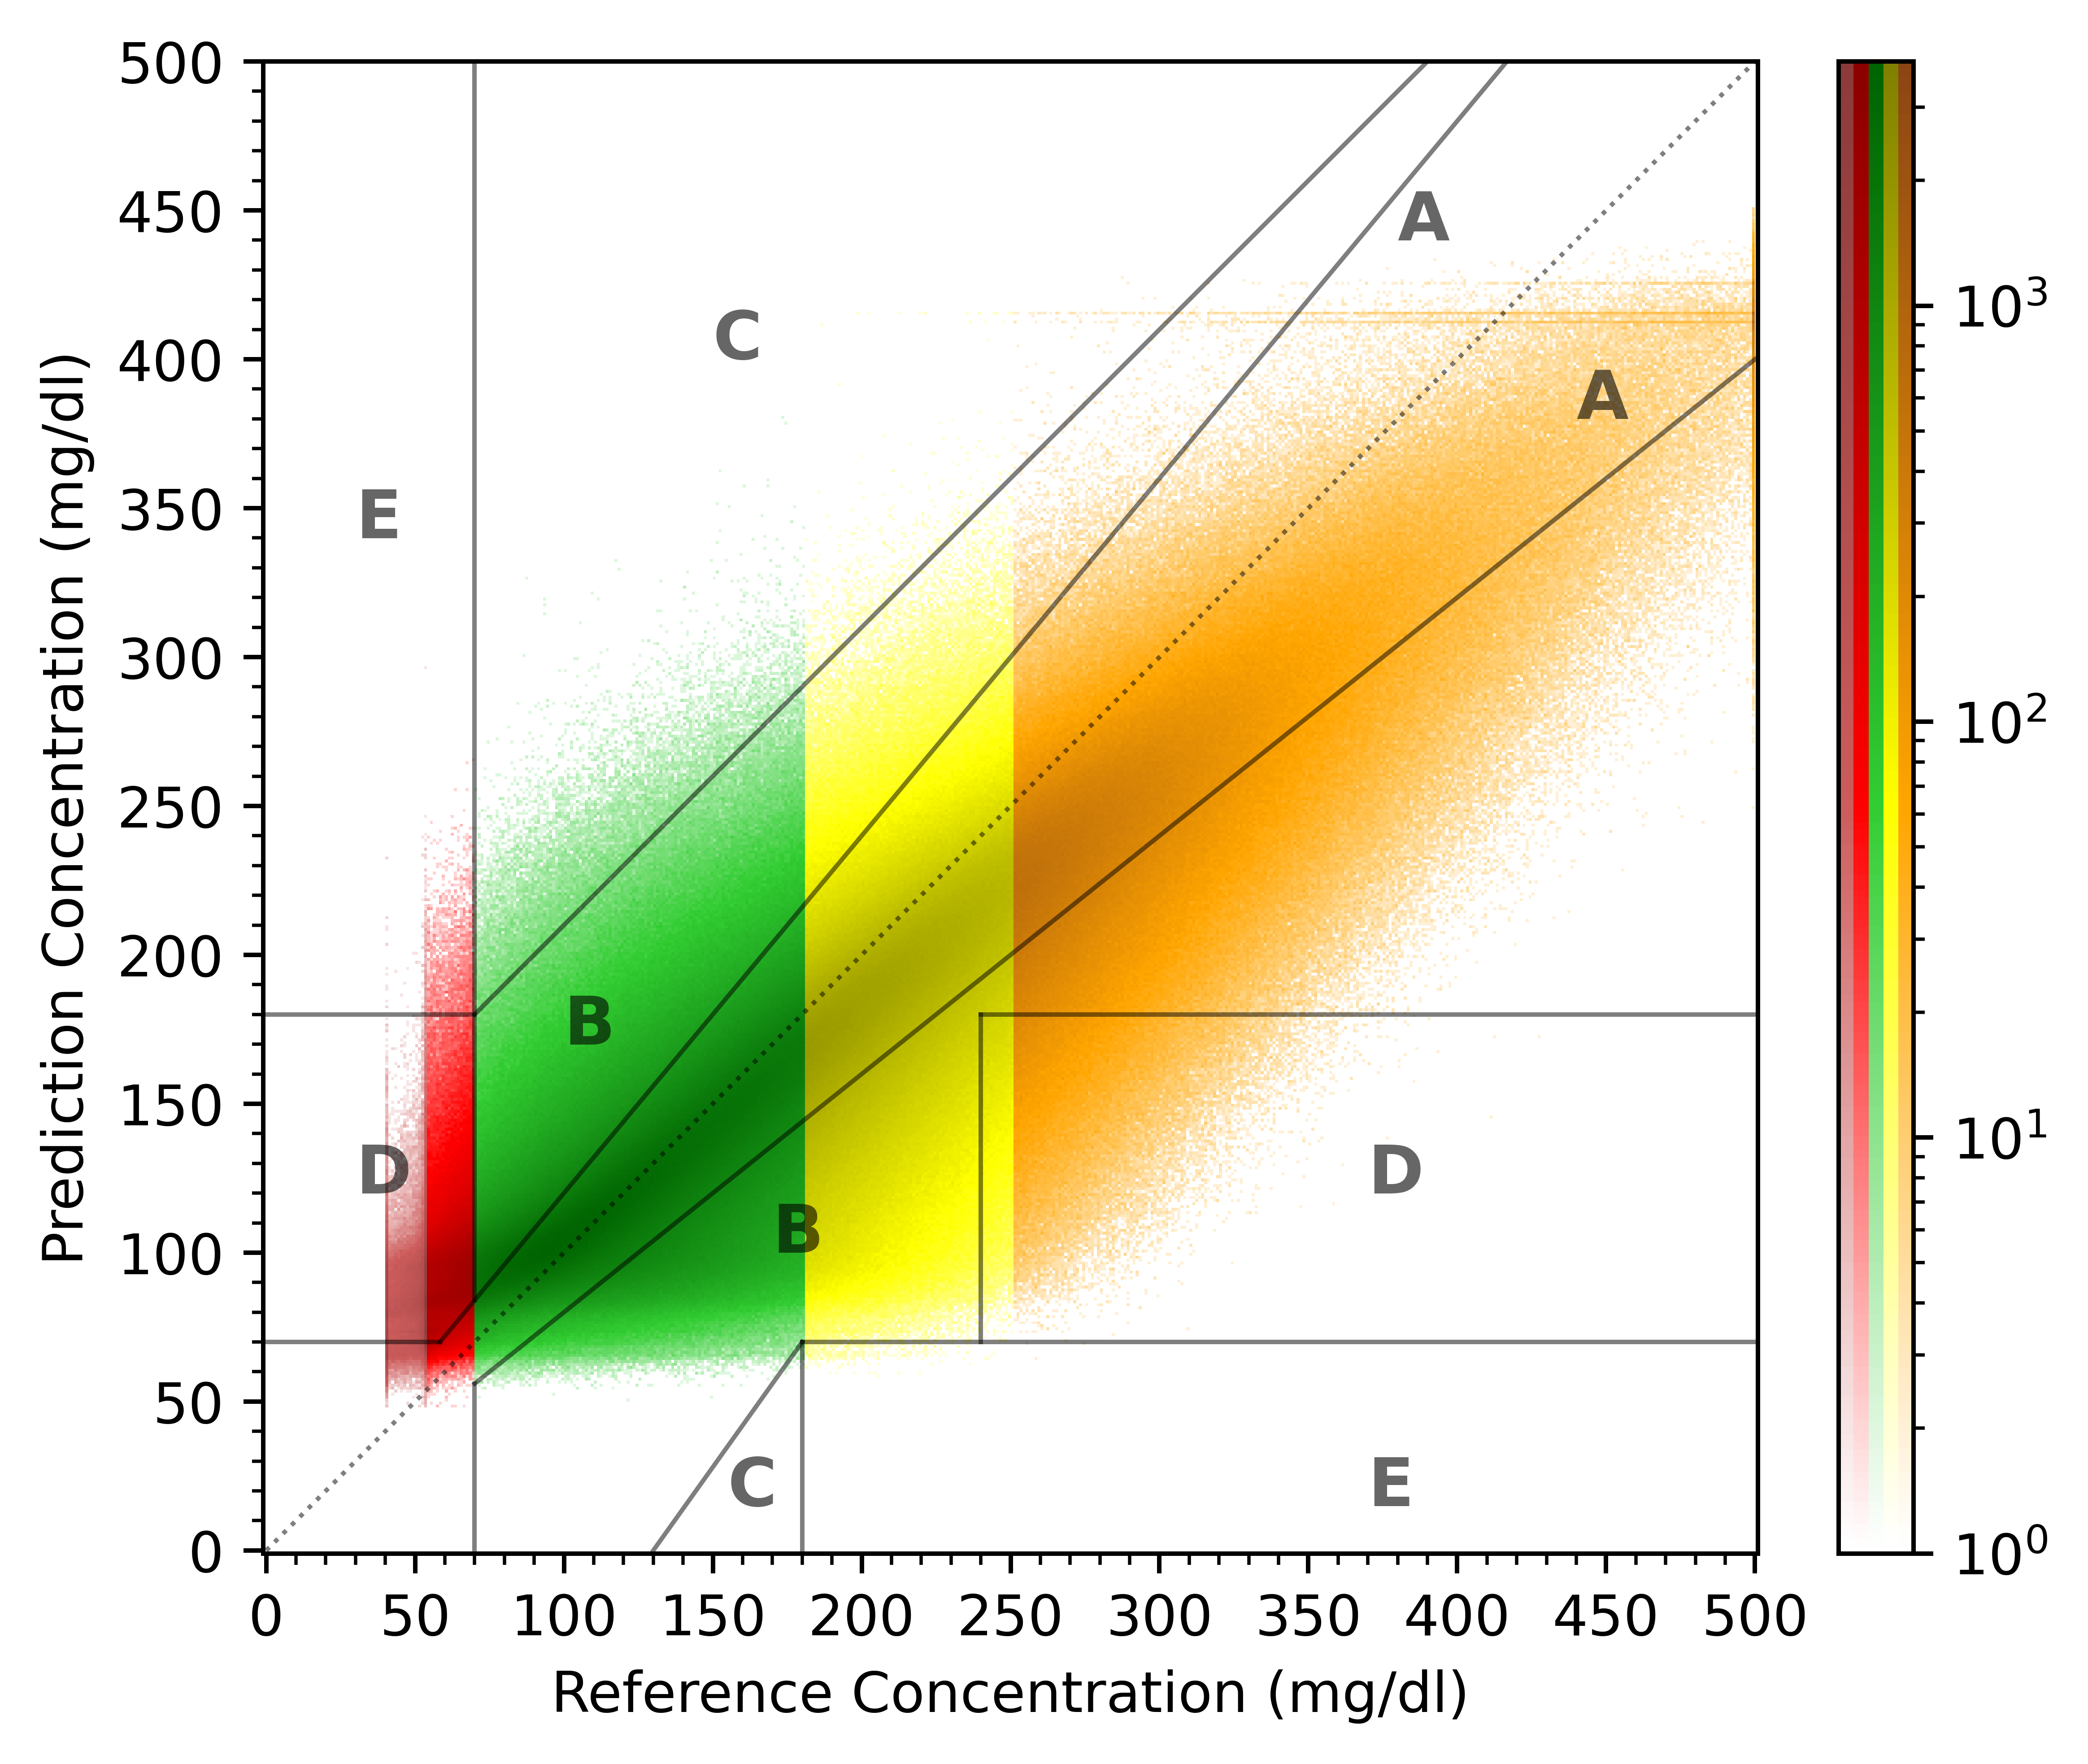
\includegraphics[width=0.82\textwidth]
    {images/CEGA_T1DiabetesGranada/T1DiabetesGranada_random_normalized.png}
    \caption{Clarke Error Grid for T1DiabetesGranada using random
    resampling and the normalized baseline target distribution.}
    \label{fig:t1diabetesgranada_clarke_normalized}
\end{figure}

\begin{figure}[htbp]
    \centering
    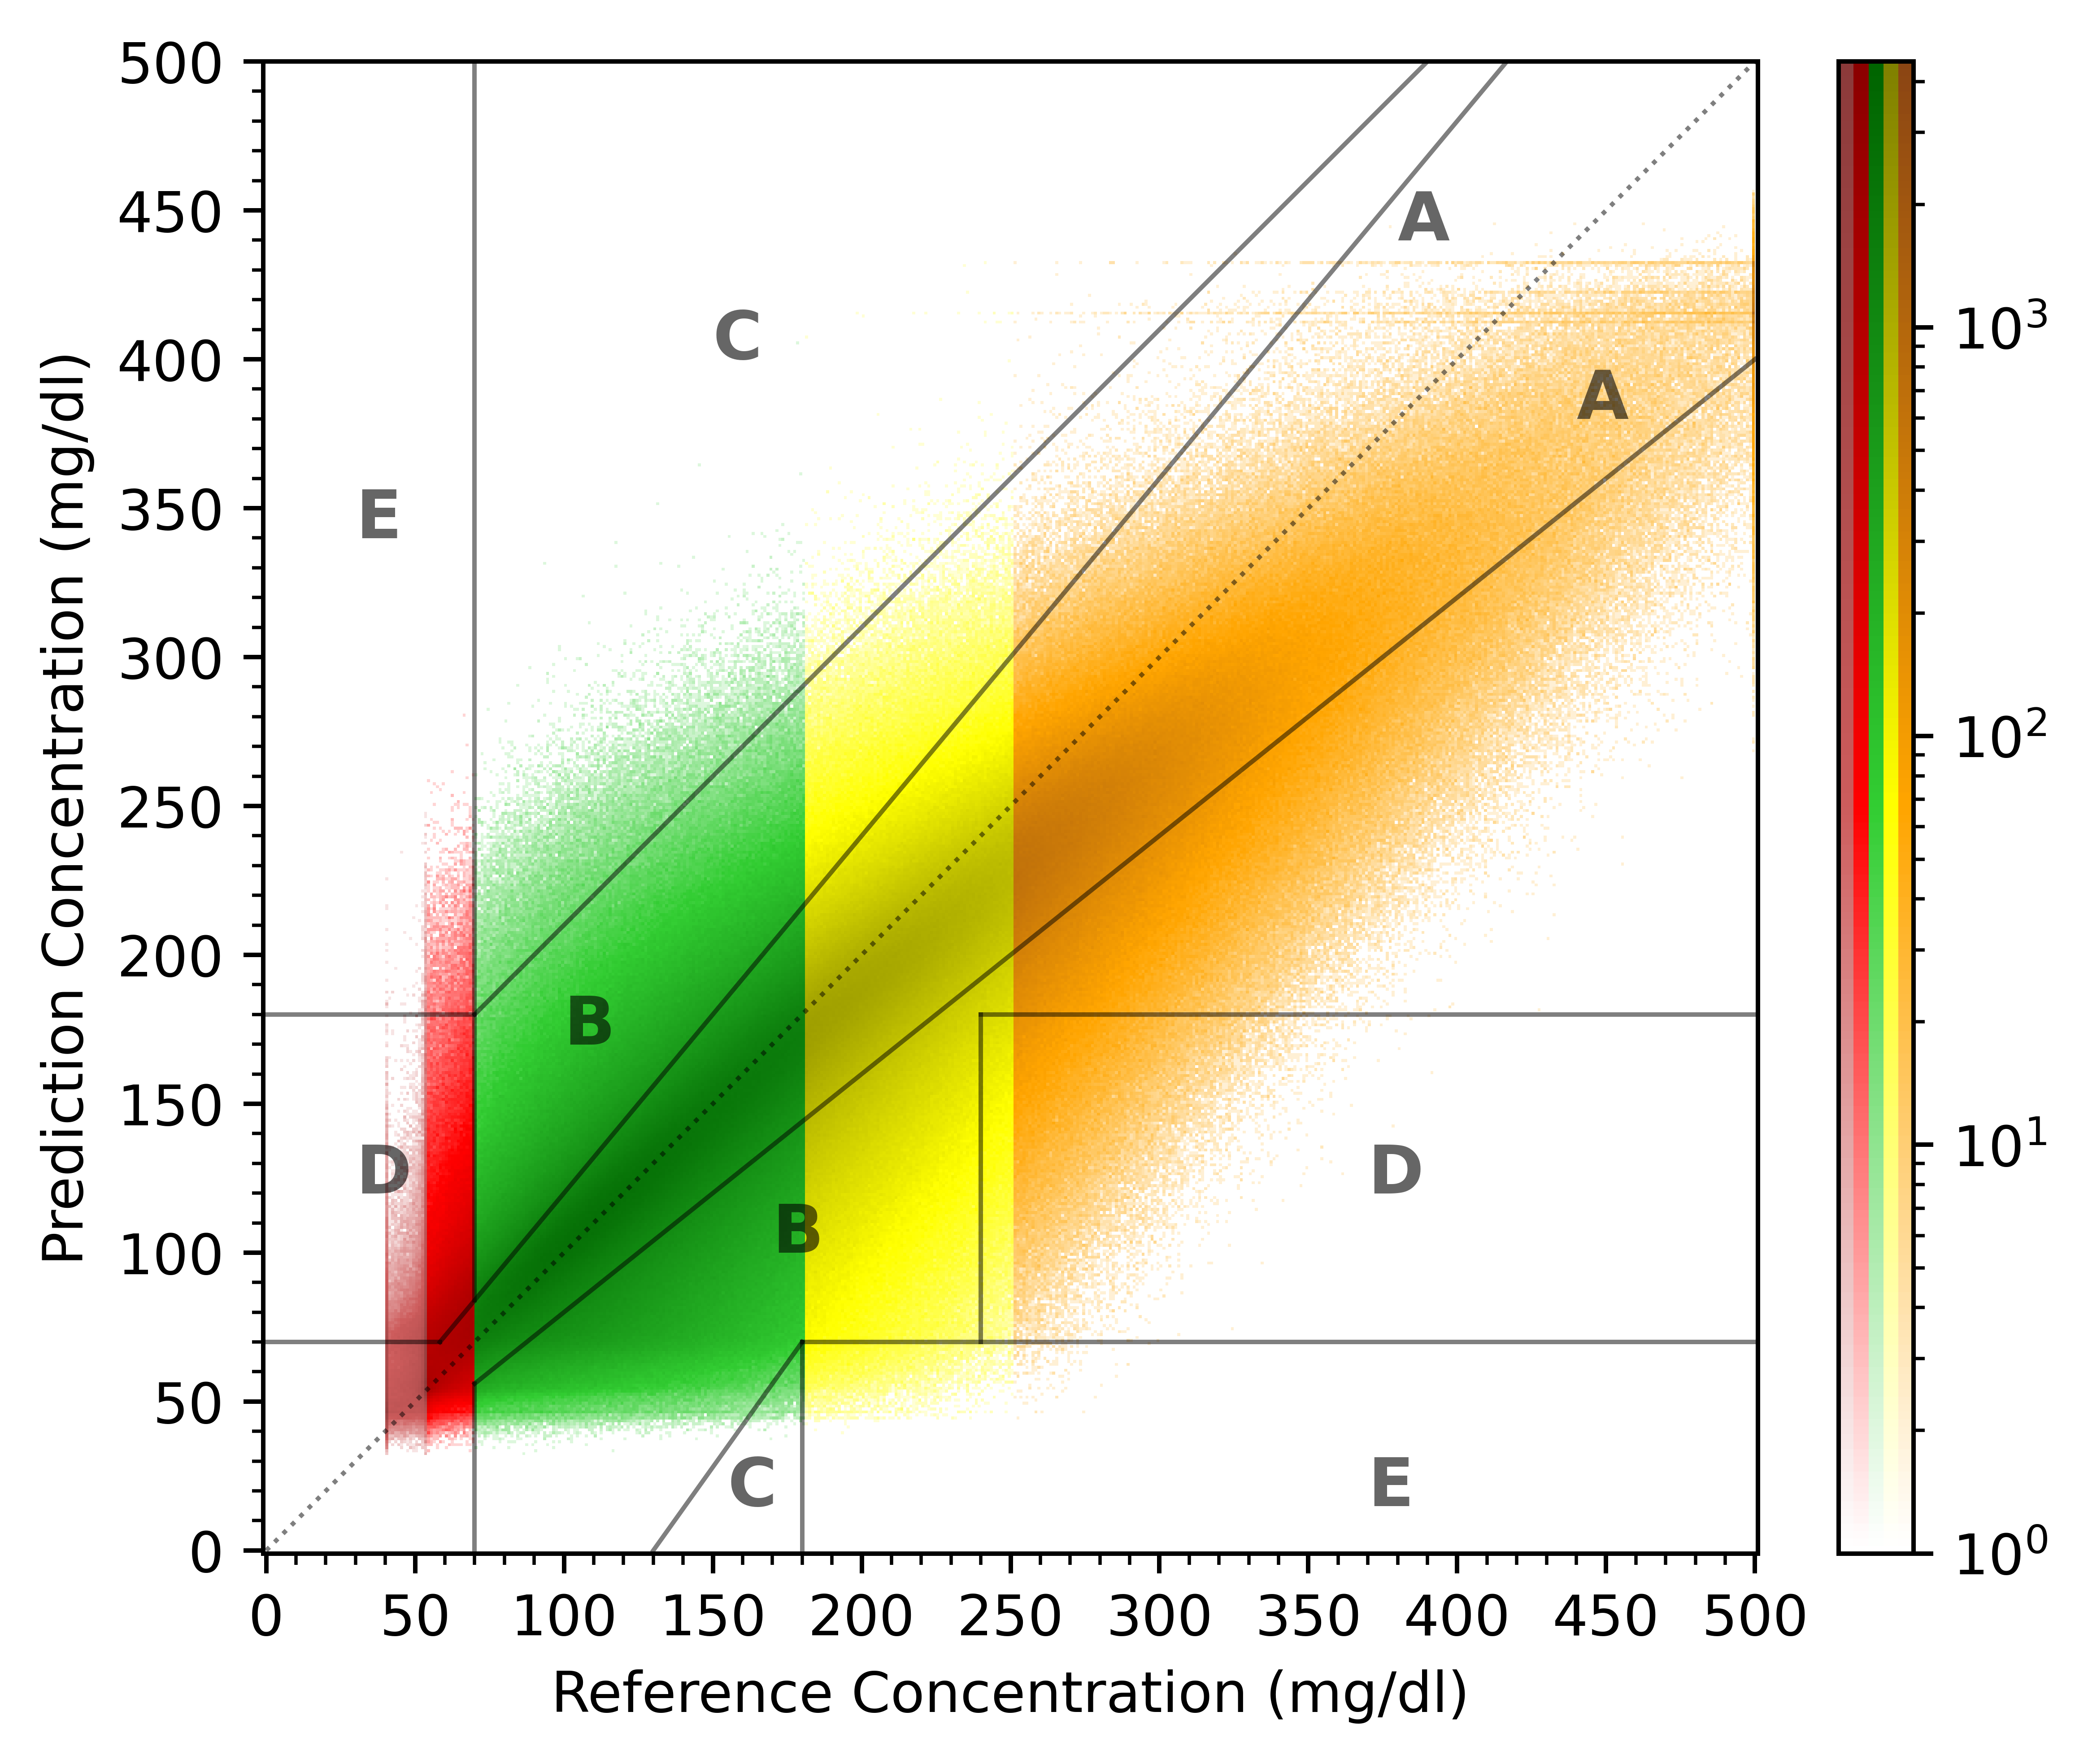
\includegraphics[width=0.82\textwidth]
    {images/CEGA_T1DiabetesGranada/T1DiabetesGranada_random_semi.png}
    \caption{Clarke Error Grid for T1DiabetesGranada using random
    resampling and the semi-balanced target distribution.}
    \label{fig:t1diabetesgranada_clarke_semi}
\end{figure}

\begin{figure}[htbp]
    \centering
    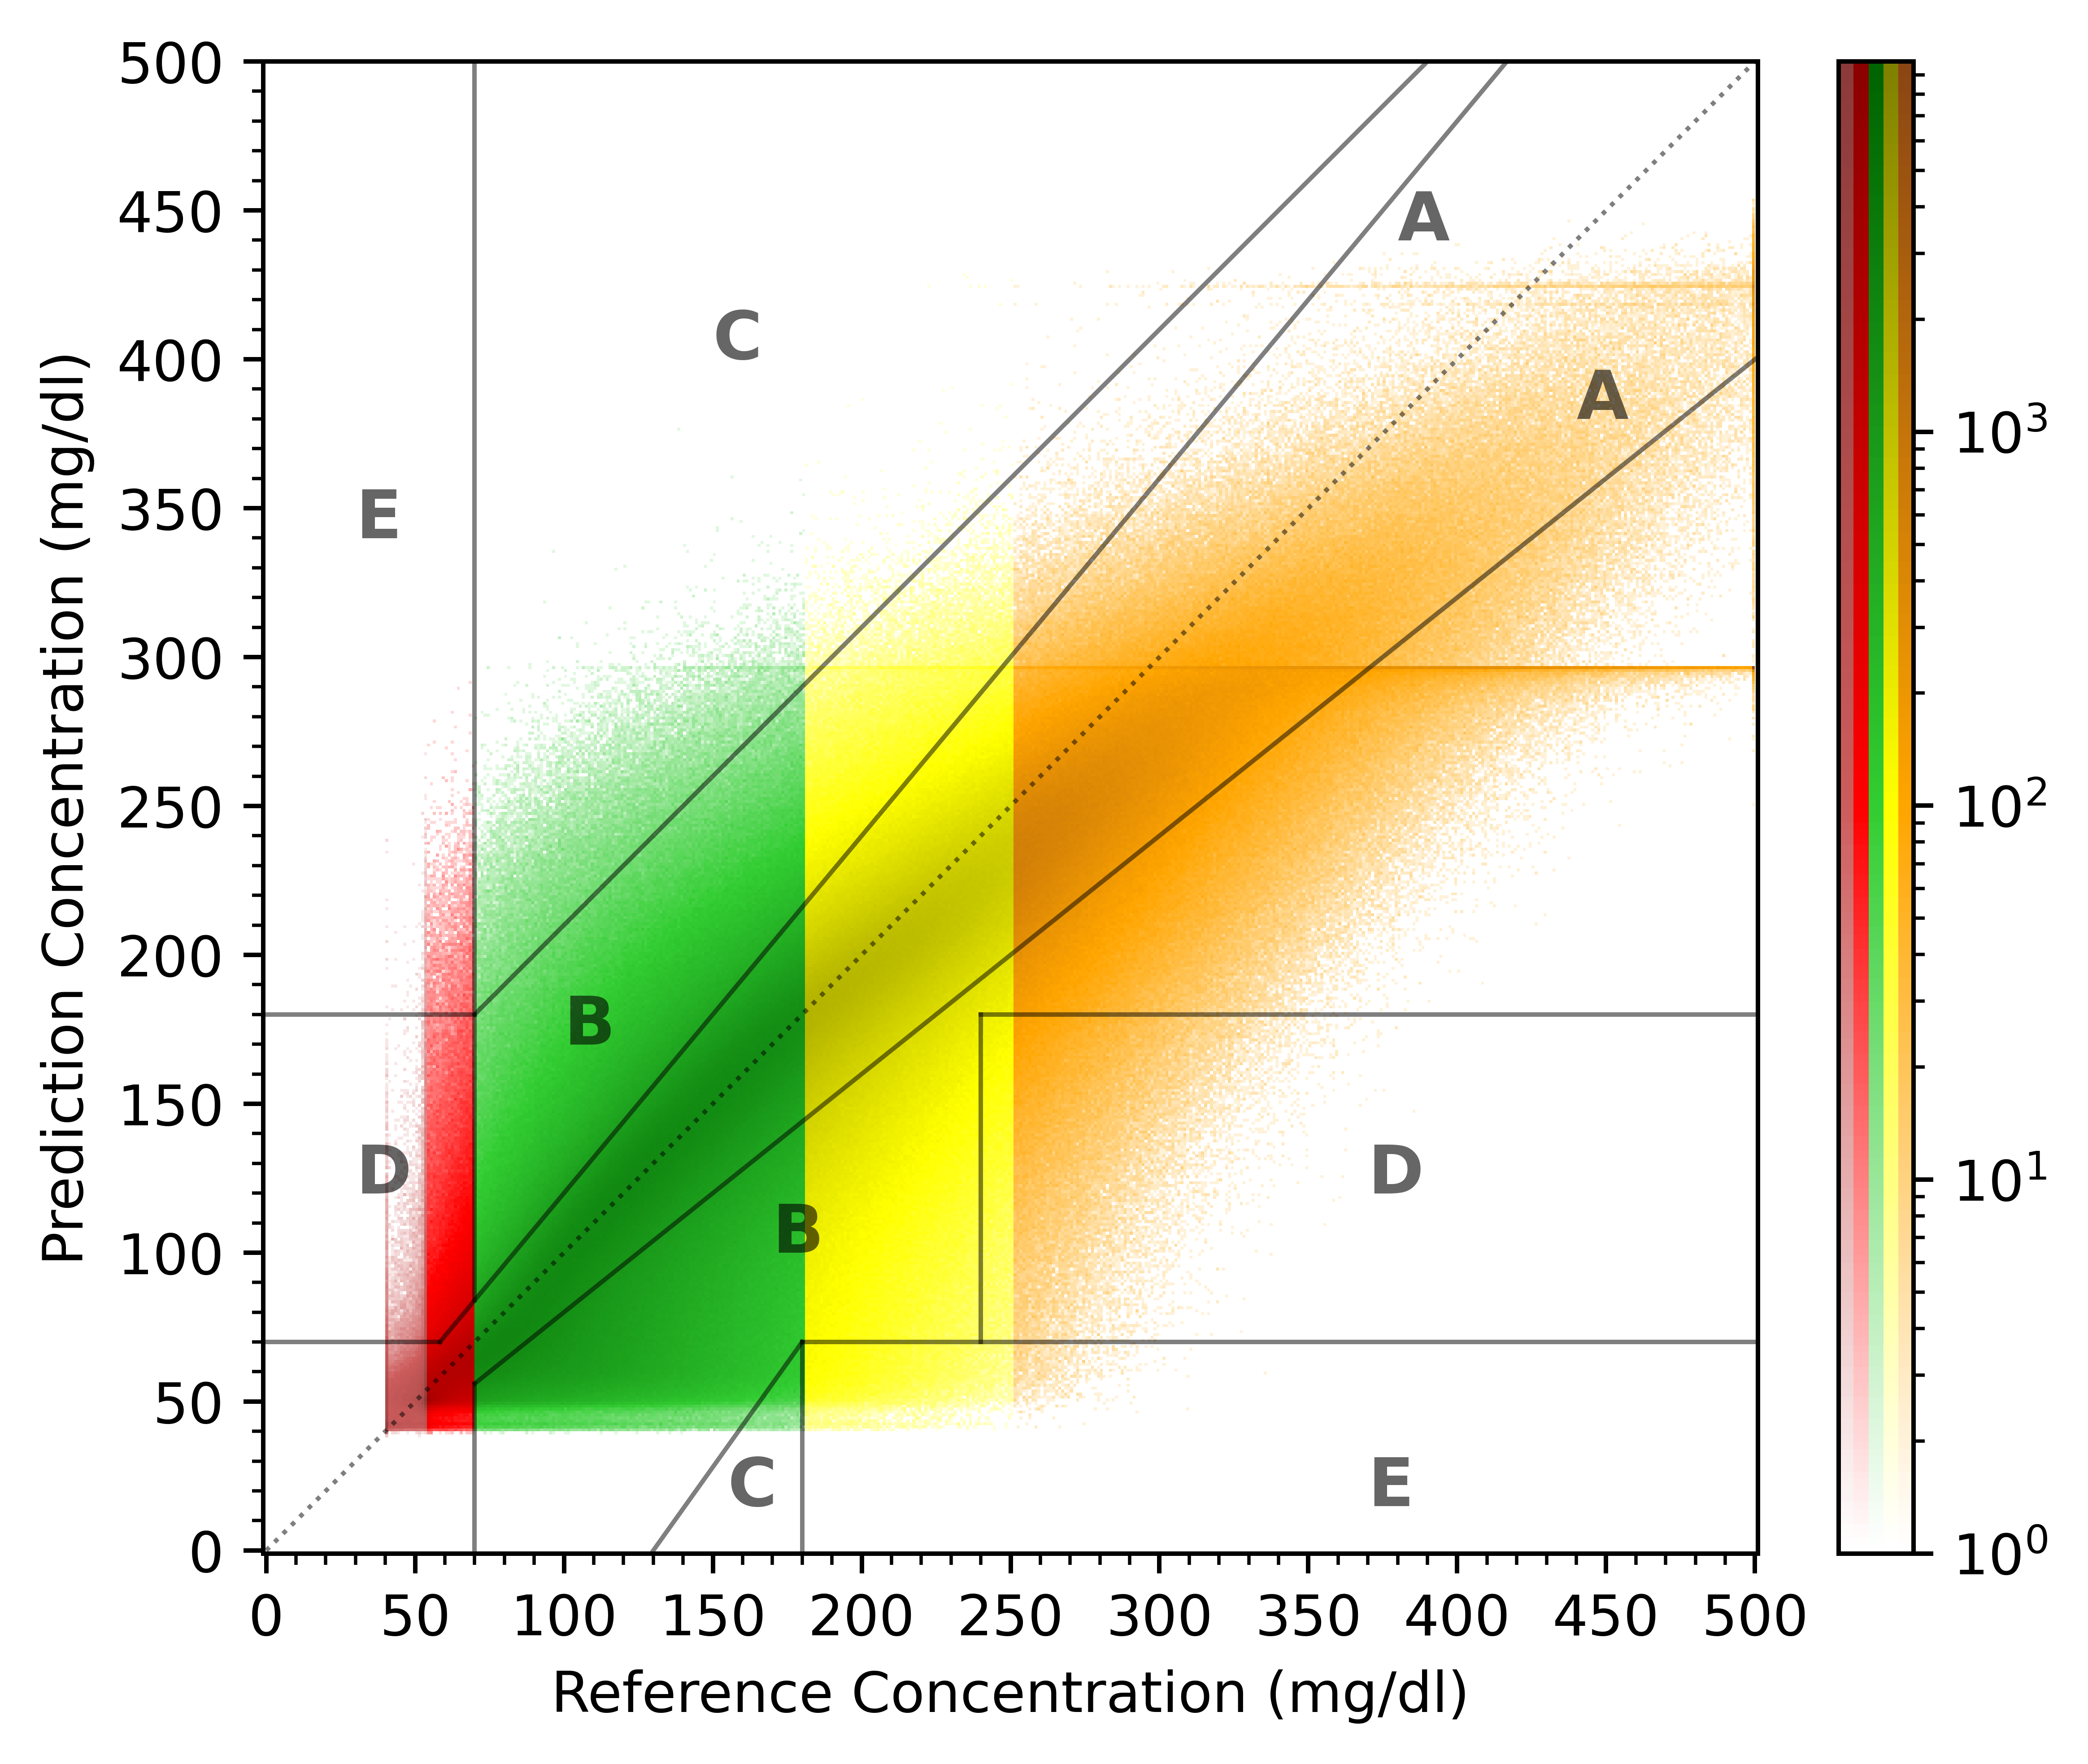
\includegraphics[width=0.82\textwidth]
    {images/CEGA_T1DiabetesGranada/T1DiabetesGranada_random_full.png}
    \caption{Clarke Error Grid for T1DiabetesGranada using random
    resampling and the fully balanced target distribution.}
    \label{fig:t1diabetesgranada_clarke_full}
\end{figure}

The grids support the same interpretation observed in the previous datasets.

\subsection{T1DiabetesGranada Summary}
\label{subsec:t1diabetesgranadasummary}

The primary statistical analysis rejected the null hypothesis for T1DiabetesGranada.

The aggregate results confirm the clinical magnitude of this effect. TBR$_2$ A+B increased from \(13.24\%\) under normalized balancing to \(88.87\%\) under full balancing, while TBR$_1$ A+B increased from \(8.47\%\) to \(79.06\%\).

The balancing method again had little descriptive influence compared with the selected target distribution. Semi-balancing provided a strong intermediate response and slightly improved global RMSE, while full balancing produced the largest improvements in both hypoglycemic ranges.

Full balancing reduced numerical precision in TIR, although TIR A+B remained above \(99\%\) and no predictions entered Zones D or E. Severe hyperglycemia also improved, while moderate hyperglycemia showed a smaller localized deterioration.

Overall, full balancing is considered the most beneficial T1DiabetesGranada configuration. Its moderate numerical cost in global performance and TIR is definitely outweighed by the magnitude and clinical relevance of the improvements obtained in TBR.

% ============================================================
% CROSS-DATASET STATISTICAL SYNTHESIS
% ============================================================

\section{Cross-Dataset Statistical Synthesis}
\label{sec:cross_dataset_statistical_synthesis}

\subsection{Comparison of the Primary Effects}
\label{subsec:primary_effect_comparison}

Table~\ref{tab:cross_dataset_primary_results} summarizes the primary statistical results across the three datasets.

\begin{table}[htbp]
\centering
\caption{Cross-dataset comparison of the primary statistical outcome.}
\label{tab:cross_dataset_primary_results}
\resizebox{\textwidth}{!}{%
\begin{tabular}{lcccc}
\toprule
\textbf{Dataset}
& $\boldsymbol{\overline{\Delta} AB_{\mathrm{TBR_2}}}$
& $\boldsymbol{t}$
& \textbf{$\boldsymbol{p}$-value}
& \textbf{Decision} \\
\midrule
DiaTrend
& $+63.75$ pp
& $11.57$
& $1.60 \times 10^{-4}$
& Reject $H_0$ \\

REPLACE-BG
& $+76.81$ pp
& $78.23$
& $8.00 \times 10^{-8}$
& Reject $H_0$ \\

T1DiabetesGranada
& $+75.93$ pp
& $30.60$
& $3.40 \times 10^{-6}$
& Reject $H_0$ \\
\bottomrule
\end{tabular}%
}
\end{table}

Full balancing produced a statistically significant improvement in all three datasets. The effects obtained for REPLACE-BG and T1DiabetesGranada were nearly identical, whereas DiaTrend showed a slightly smaller and more variable, although still substantial, improvement.

\subsection{Holm-Adjusted Statistical Results}
\label{subsec:holm_adjusted_results}

Since the primary hypothesis was evaluated independently in three datasets, the corresponding $p$-values were adjusted using the Holm procedure \cite{enwiki:1352765388}.

\begin{table}[htbp]
\centering
\caption{Original and Holm-adjusted $p$-values for the primary outcome.}
\label{tab:holm_adjusted_primary_results}
\begin{tabular}{lccc}
\toprule
\textbf{Dataset}
& \textbf{Original $p$-value}
& \textbf{Holm-adjusted $p$-value}
& \textbf{Decision} \\
\midrule
DiaTrend
& $1.60 \times 10^{-4}$
& $1.60 \times 10^{-4}$
& Reject $H_0$ \\

REPLACE-BG
& $8.00 \times 10^{-8}$
& $2.40 \times 10^{-7}$
& Reject $H_0$ \\

T1DiabetesGranada
& $3.40 \times 10^{-6}$
& $6.80 \times 10^{-6}$
& Reject $H_0$ \\
\bottomrule
\end{tabular}
\end{table}

All adjusted $p$-values still remained below the predefined significance level of $\alpha = 0.01$. Therefore, the correction did not alter any of the dataset-specific conclusions.

\subsection{Consistency of the Primary Outcome}
\label{subsec:primary_outcome_consistency}

The primary effect was therefore consistent across the three datasets: full balancing improved $AB_{\mathrm{TBR_2}}$ in every fold and in all individual method--fold comparisons. Apart from the slightly smaller effect observed in DiaTrend, the results were analogous and consistently supported the primary hypothesis.

% ============================================================
% CROSS-DATASET SECONDARY-OUTCOMES SYNTHESIS
% ============================================================

\section{Cross-Dataset Secondary-Outcomes Synthesis}
\label{sec:cross_dataset_secondary_synthesis}

\subsection{Influence of the Target Distribution}
\label{subsec:cross_dataset_target_effect}

The three datasets showed the same general relationship between balancing intensity and predictive performance. Semi-balancing provided an intermediate response, and full balancing produced the largest clinical improvements. Therefore, the selected target distribution was consistently the principal factor determining the effect of balancing.

\subsection{Influence of the Balancing Method}
\label{subsec:cross_dataset_method_effect}

Random resampling, SMOTER, and SMOGN produced analogous results in all three datasets. The variability between methods remained considerably smaller than the differences between target distributions, indicating that balancing intensity had a substantially greater influence than the particular resampling method.

\subsection{Hypoglycemic Performance Across Datasets}
\label{subsec:cross_dataset_hypoglycemia}

Hypoglycemic performance improved progressively from normalized to semi-balanced and fully balanced configurations in every dataset, consistently reproducing the relationship suggested in Equation~\ref{eq:ordered_hypothesis_conjecture}.

The main difference was observed in T1DiabetesGranada, where semi-balancing already produced a particularly strong improvement and full balancing reached the highest final TBR$_2$ A+B value. Nevertheless, full balancing produced substantial improvements in both TBR$_2$ and TBR$_1$ across all datasets, mainly through a redistribution of predictions from Zone D into Zone A.

\subsection{Global Accuracy and Time-in-Range Trade-Off}
\label{subsec:cross_dataset_global_tradeoff}

The global and TIR trade-offs were also analogous. Semi-balancing largely preserved global numerical accuracy, whereas full balancing increased global and TIR errors. This deterioration was largest in REPLACE-BG and smallest in T1DiabetesGranada.

Despite the numerical deterioration, global A+B increased in every dataset. TIR A+B remained above (99\%), and no TIR predictions entered Zones D or E. Consequently, the cost of full balancing was predominantly numerical, while its global clinical performance remained stable or improved.

\subsection{Hyperglycemic Performance Across Datasets}
\label{subsec:cross_dataset_hyperglycemia}

The hyperglycemic results followed the same pattern across the three datasets. Semi-balancing had a neutral or slightly positive effect in TAR$_1$, while both semi and full balancing improved numerical and clinical performance in TAR$_2$.

Full balancing introduced a localized deterioration in TAR$_1$, including a small increase in Zone E. This effect was most pronounced in DiaTrend and smallest in T1DiabetesGranada. Nevertheless, it remained substantially smaller than the improvements obtained in the hypoglycemic ranges, while severe hyperglycemia consistently benefited from balancing.
